% !TEX program = xelatex
% ============================================================================
% មគ្គុទ្ទេសក៍គរុកោសល្យគ្រូ និងសេណារីយ៉ូបង្រៀនលម្អិត (Teacher's Guideline -- PB)
% មុខវិជ្ជា៖ គណិតវិទ្យា ថ្នាក់ទី៨ -- មេរៀនទី១២៖ ការប្រៀបធៀបត្រីកោណ
% ចំណុចរង៖ ២.១ លក្ខណៈមេដ្យាទ័រនៃអង្កត់ (សៀវភៅគោល ទំ.១៥៦ និង ១៦៤: #1, #3, #5)
% គ្រូបង្រៀន៖ ហុក ប៊ុនថែន | អនុវិទ្យាល័យព្រះក្រសាំង (កំពង់ស្វាយ-កំពង់ធំ)
% ============================================================================
\documentclass[a4paper,12pt]{article}

\usepackage[a4paper, left=1.55cm, right=1.55cm, top=2.30cm, bottom=2.30cm, headheight=20pt, headsep=0.68cm, footskip=0.88cm]{geometry}
\usepackage{amsmath, amssymb}
\usepackage{unicode-math}
\usepackage{fontspec}
\usepackage{array, longtable, multirow, colortbl, booktabs}
\usepackage[table]{xcolor}
\usepackage{enumitem}
\usepackage{pifont}
\usepackage{fancyhdr}
\usepackage{lastpage}
\usepackage{needspace}
\usepackage[hyphens]{url}
\usepackage{tikz}
\usepackage[most]{tcolorbox}
\usetikzlibrary{calc, arrows.meta, angles, quotes, decorations.markings, positioning, babel}
\urlstyle{same}

\makeatletter
\let\@expl@@@mark@update@singlecol@structures@@\relax
\makeatother

% ============================================================================
% ការកំណត់ពុម្ពអក្សរ (Word-Styled Khmer + Times New Roman APA + Cambria Math)
% ============================================================================
% Cross-platform font path resolver (Windows local + Linux/Cloud repo fonts/)
\providecommand{\NGSFindFonts}{%
  \IfFileExists{C:/Windows/Fonts/cambria.ttc}{%
    \def\NGSSysPath{C:/Windows/Fonts/}%
    \def\NGSUserPath{C:/Users/KIT/AppData/Local/Microsoft/Windows/Fonts/}%
  }{%
    \IfFileExists{./fonts/KhmerOSsiemreap.ttf}{\def\NGSSysPath{./fonts/}\def\NGSUserPath{./fonts/}}{%
    \IfFileExists{../fonts/KhmerOSsiemreap.ttf}{\def\NGSSysPath{../fonts/}\def\NGSUserPath{../fonts/}}{%
    \IfFileExists{../../fonts/KhmerOSsiemreap.ttf}{\def\NGSSysPath{../../fonts/}\def\NGSUserPath{../../fonts/}}{%
    \IfFileExists{../../../fonts/KhmerOSsiemreap.ttf}{\def\NGSSysPath{../../../fonts/}\def\NGSUserPath{../../../fonts/}}{%
    \IfFileExists{../../../../fonts/KhmerOSsiemreap.ttf}{\def\NGSSysPath{../../../../fonts/}\def\NGSUserPath{../../../../fonts/}}{%
    \IfFileExists{../../../../../fonts/KhmerOSsiemreap.ttf}{\def\NGSSysPath{../../../../../fonts/}\def\NGSUserPath{../../../../../fonts/}}{%
    \IfFileExists{../../../../../../fonts/KhmerOSsiemreap.ttf}{\def\NGSSysPath{../../../../../../fonts/}\def\NGSUserPath{../../../../../../fonts/}}{%
      \def\NGSSysPath{../../../../../../../fonts/}\def\NGSUserPath{../../../../../../../fonts/}%
    }}}}}}}%
  }%
}
\NGSFindFonts

\setmathfont[
  Path={\NGSSysPath},
  FontIndex=1,
  Scale=1.06
]{cambria.ttc}

\defaultfontfeatures{Ligatures=TeX}

\setmainfont[
  Path={\NGSUserPath},
  Extension=.ttf,
  Script=Khmer,
  BoldFont={KhmerOSsiemreap},
  BoldFeatures={FakeBold=1.8},
  ItalicFont={KhmerOSsiemreap},
  ItalicFeatures={FakeSlant=0.25},
  BoldItalicFont={KhmerOSsiemreap},
  BoldItalicFeatures={FakeBold=1.8, FakeSlant=0.25}
]{KhmerOSsiemreap}

% ហាមដាក់ FakeBold លើ KhmerOSmuollight និងកុំរុំ \muol ក្នុង \textbf{...}
\newfontfamily\muol[
  Path={\NGSUserPath},
  Extension=.ttf,
  Script=Khmer
]{KhmerOSmuollight}

\newfontfamily\TimesEn[
  Path={\NGSSysPath},
  Extension=.ttf,
  Scale=1.02,
  BoldFont={timesbd},
  ItalicFont={timesi},
  BoldItalicFont={timesbi}
]{times}

\newfontfamily\Tacteing[
  Path={\NGSUserPath}
]{TACTENG.TTF}

\newfontfamily\CourierBullet[
  Path={\NGSSysPath},
  Extension=.ttf
]{cour}

% ក្បួនកាត់ពាក្យខ្មែរ (Khmer word wrapping)
\XeTeXlinebreaklocale "km"
\XeTeXlinebreakskip = 0pt plus 1pt minus 0.1pt

% Mobile-First comfortable line spacing (11.5pt / 18.2pt effective)
\linespread{1.22}

% ============================================================================
% ពណ៌ ស-ខ្មៅ (Strict Monochrome Grayscale Palette) & Fancyhdr
% ============================================================================
\definecolor{headgray}{HTML}{F2F2F2}
\definecolor{panelgray}{gray}{0.94}
\definecolor{stepgray}{HTML}{D9D9D9}
\definecolor{midgray}{gray}{0.82}
\definecolor{bordergray}{gray}{0.45}

\pagestyle{fancy}
\fancyhf{}
\renewcommand{\headrulewidth}{0.4pt}
\renewcommand{\footrulewidth}{0.4pt}
\fancyhead[L]{\rule[-3pt]{0pt}{14pt}\fontsize{9.8pt}{13.5pt}\selectfont អនុវិទ្យាល័យព្រះក្រសាំង \en{---} មគ្គុទ្ទេសក៍គរុកោសល្យគ្រូ \en{(Grade 8 PB)}}
\fancyhead[R]{\rule[-3pt]{0pt}{14pt}\fontsize{9.8pt}{13.5pt}\selectfont មេរៀនទី១២ \en{(}២.១\en{)} លក្ខណៈមេដ្យាទ័រនៃអង្កត់}
\fancyfoot[L]{\rule{0pt}{13pt}\fontsize{9.8pt}{13.5pt}\selectfont កញ្ចប់ឯកសារ \en{NGS 5Es} \en{(}៥០ នាទី\en{)} \en{|} ហុក ប៊ុនថែន}
\fancyfoot[R]{\rule{0pt}{13pt}\fontsize{9.8pt}{13.5pt}\selectfont ទំព័រ \en{\thepage\ / \pageref{LastPage}}}

\fancypagestyle{firstpage}{%
  \fancyhf{}%
  \renewcommand{\headrulewidth}{0pt}%
  \renewcommand{\footrulewidth}{0.4pt}%
  \fancyfoot[L]{\rule{0pt}{13pt}\fontsize{9.8pt}{13.5pt}\selectfont កញ្ចប់ឯកសារ \en{NGS 5Es} \en{(}៥០ នាទី\en{)} \en{|} អនុវិទ្យាល័យព្រះក្រសាំង}%
  \fancyfoot[R]{\rule{0pt}{13pt}\fontsize{9.8pt}{13.5pt}\selectfont ទំព័រ \en{\thepage\ / \pageref{LastPage}}}%
}

\setlength{\parindent}{0pt}
\setlength{\parskip}{3.0pt}
\setlength{\tabcolsep}{4pt}
\setlength{\emergencystretch}{2em}
\setlist{itemsep=2.5pt, parsep=0pt}

% ============================================================================
% ម៉ាក្រូជំនួយ និងឋានានុក្រម \muol គ្មានតួអក្សរ ASCII បន្លំ
% ============================================================================
\newcommand{\en}[1]{{\TimesEn #1}}
\newcommand{\enbf}[1]{{\TimesEn\textbf{#1}}}
\newcommand{\enit}[1]{{\TimesEn\textit{#1}}}
\newcommand{\unit}[1]{\,\text{\en{#1}}}
\newcommand{\cnum}[1]{{\TimesEn\fontsize{10.5pt}{12pt}\selectfont\ding{\numexpr181+#1\relax}}}
\newcommand{\ditem}{\tikz[baseline=-0.5ex]\fill (0,0.40ex) -- (0.40ex,0) -- (0,-0.40ex) -- (-0.40ex,0) -- cycle;\hspace{0.25em}}
\newcommand{\wcirc}{{\CourierBullet\fontsize{9.8pt}{11pt}\selectfont o}}
\newcommand{\chkbox}{\tikz[baseline=-0.15ex]\draw[black, line width=0.85pt] (0,0) rectangle (0.25cm,0.25cm);}
\newcommand{\tri}[1]{\ensuremath{\triangle #1}}
\newcommand{\ang}[1]{\ensuremath{\angle #1}}
\newcommand{\cg}{\ensuremath{\cong}}
\newcommand{\ncg}{\ensuremath{\not\cong}}
\newcommand{\khmflourish}{{\Tacteing\fontsize{38pt}{15pt}\selectfont\raisebox{-5pt}{3}}}
\newcommand{\tickone}{\tikz[baseline=-0.2ex]\draw[black, line width=1.1pt] (0,0) -- (0,0.24cm);}
\newcommand{\ticktwo}{\tikz[baseline=-0.2ex]{\draw[black, line width=1.1pt] (0,0) -- (0,0.24cm);\draw[black, line width=1.1pt] (0.08cm,0) -- (0.08cm,0.24cm);}}
\newcommand{\tickslash}{\tikz[baseline=-0.2ex]\draw[black, line width=1.1pt] (0,0) -- (0.12cm,0.22cm);}
\newcommand{\tickcross}{\tikz[baseline=-0.2ex]{\draw[black, line width=1.1pt] (0,0) -- (0.18cm,0.20cm);\draw[black, line width=1.1pt] (0,0.20cm) -- (0.18cm,0);}}

\newcommand{\parttitle}[1]{{\muol\fontsize{13pt}{17pt}\selectfont #1}}
\newcommand{\sectitle}[1]{{\muol\fontsize{12pt}{15.5pt}\selectfont #1}}
\newcommand{\subsectitle}[1]{{\muol\fontsize{11pt}{14.5pt}\selectfont #1}}
\newcommand{\tblhead}[1]{{\muol\fontsize{10.5pt}{16.2pt}\selectfont #1\par}}

\newcolumntype{L}[1]{>{\raggedright\arraybackslash}p{#1}}
\newcolumntype{C}[1]{>{\centering\arraybackslash}p{#1}}
\newcolumntype{R}[1]{>{\raggedleft\arraybackslash}p{#1}}

\newcommand{\secbanner}[2]{%
  \Needspace{6.5cm}%
  \vspace{2pt}%
  \begin{tcolorbox}[
    enhanced, sharp corners, colback=stepgray, colframe=black,
    boxrule=1.1pt, borderline south={0.6pt}{1.8pt}{black},
    top=5pt, bottom=5pt, left=9pt, right=9pt,
    before skip=6pt, after skip=5pt
  ]
    \sectitle{#1}\\[2pt]
    {\fontsize{10pt}{12.5pt}\selectfont\enit{#2}}%
  \end{tcolorbox}%
}

\newcommand{\subsec}[1]{%
  \Needspace{4.5cm}%
  \vspace{4pt}%
  \subsectitle{#1}\par%
  \vspace{-2pt}%
  {\color{black}\hrule height 0.55pt}%
  \vspace{3.5pt}%
}

\newtcolorbox{phasebox}[3]{%
  enhanced, breakable, sharp corners, colback=white, colframe=black,
  boxrule=1.0pt, top=5pt, bottom=5pt, left=9pt, right=9pt,
  toptitle=3.5pt, bottomtitle=3.5pt,
  before skip=6pt, after skip=5pt,
  colbacktitle=headgray, coltitle=black,
  fonttitle=\fontsize{11pt}{14.5pt}\selectfont,
  fontupper=\fontsize{11.5pt}{14.92pt}\selectfont,
  title={%
    \linespread{1.0}\selectfont\renewcommand{\arraystretch}{1.0}%
    \begin{tabular*}{\linewidth}{@{}>{\raggedright\arraybackslash}p{12.80cm}@{\extracolsep{\fill}}r@{}}
      {\muol\fontsize{11pt}{14.5pt}\selectfont #1} & {\fontsize{10.5pt}{13.5pt}\selectfont\en{#2 |} #3}%
    \end{tabular*}%
  }
}

\newtcolorbox{scriptbox}{%
  enhanced, breakable, sharp corners, colback=panelgray, colframe=black,
  boxrule=0.6pt, borderline west={2.4pt}{0pt}{black},
  top=4pt, bottom=4pt, left=9pt, right=8pt,
  before skip=3pt, after skip=3pt,
  fontupper=\fontsize{11.5pt}{14.92pt}\selectfont
}

\tikzset{
  tk1/.style={postaction={decorate}, decoration={markings, mark=at position 0.5 with {\draw[black, line width=0.95pt] (0,-0.12) -- (0,0.12);}}},
  tk2/.style={postaction={decorate}, decoration={markings,
    mark=at position 0.45 with {\draw[black, line width=0.95pt] (0,-0.12) -- (0,0.12);},
    mark=at position 0.55 with {\draw[black, line width=0.95pt] (0,-0.12) -- (0,0.12);}}},
  tkslash/.style={postaction={decorate}, decoration={markings, mark=at position 0.5 with {\draw[black, line width=0.95pt] (-0.075,-0.10) -- (0.075,0.10);}}},
  tkcross/.style={postaction={decorate}, decoration={markings, mark=at position 0.5 with {
    \draw[black, line width=0.95pt] (-0.085,-0.085) -- (0.085,0.085);
    \draw[black, line width=0.95pt] (-0.085,0.085) -- (0.085,-0.085);}}},
  hypArrow/.style={black, densely dashed, line width=0.85pt, -{Stealth[length=4pt]}},
  ang1/.style={draw=black, line width=0.8pt}
}

\newcommand{\rightanglemark}[4][0.22]{%
  % #2 = vertex, #3 = point on ray 1, #4 = point on ray 2
  \coordinate (raA) at ($#2!#1cm!#3$);
  \coordinate (raB) at ($#2!#1cm!#4$);
  \coordinate (raC) at ($(raA)+(raB)-#2$);
  \draw[line width=0.8pt, black] (raA) -- (raC) -- (raB);
}

\begin{document}
\thispagestyle{firstpage}
\fontsize{11.5pt}{14.92pt}\selectfont
\vspace*{-0.75cm}

% ============================================================================
% ក្បាលលិខិតផ្លូវការថ្នាក់ជាតិ & សាលារៀន (Kampong Thom / Kampong Svay / Preah Krasang)
% ============================================================================
{\linespread{1.08}\selectfont
\begin{center}
  {\muol\fontsize{12pt}{15.5pt}\selectfont ព្រះរាជាណាចក្រកម្ពុជា}\\[2pt]
  {\muol\fontsize{12pt}{15.5pt}\selectfont ជាតិ សាសនា ព្រះមហាក្សត្រ}\\[1pt]
  \khmflourish
\end{center}
\vspace{-4pt}
{\muol\fontsize{10.8pt}{15.5pt}\selectfont
  មន្ទីរអប់រំ យុវជន និងកីឡា ខេត្តកំពង់ធំ\\
  ការិយាល័យអប់រំ យុវជន និងកីឡា ស្រុកកំពង់ស្វាយ\\
  អនុវិទ្យាល័យព្រះក្រសាំង\par}
\vspace{4pt}
\begin{center}
  \parttitle{មគ្គុទ្ទេសក៍គរុកោសល្យគ្រូ និងសេណារីយ៉ូបង្រៀនលម្អិត \enbf{(Teacher's Guideline)}}\\[3pt]
  {\fontsize{11.2pt}{15pt}\selectfont\textbf{មេរៀនទី១២៖ ការប្រៀបធៀបត្រីកោណ \en{---} ២. មេដ្យាទ័រនៃអង្កត់និងត្រីកោណសមបាទ \en{---} ២.១ លក្ខណៈមេដ្យាទ័រនៃអង្កត់}}
\end{center}
}

\vspace{2pt}
\begin{tcolorbox}[
  enhanced, sharp corners, colback=headgray, colframe=black,
  boxrule=0.85pt, top=5pt, bottom=5pt, left=7pt, right=7pt,
  before skip=2pt, after skip=6pt
]
  \linespread{1.10}\fontsize{10.5pt}{14pt}\selectfont
  \renewcommand{\arraystretch}{1.18}
  \begin{tabular}{@{}L{3.10cm}@{}C{0.25cm}@{}L{5.55cm}@{\hspace{0.25cm}}L{2.70cm}@{}C{0.25cm}@{}L{5.00cm}@{}}
    \textbf{\en{-} មុខវិជ្ជា \en{/} ថ្នាក់} & \en{:} & គណិតវិទ្យា \en{(}ថ្នាក់ទី៨\en{)} & \textbf{\en{-} កាលបរិច្ឆេទ} & \en{:} & ថ្ងៃអង្គារ ទី១ ខែធ្នូ ឆ្នាំ២០២៦ \\
    \textbf{\en{-} ជំពូក \en{/} មេរៀន} & \en{:} & ធរណីមាត្រ \en{/} មេរៀនទី១២ & \textbf{\en{-} រយៈពេល} & \en{:} & ៥០ នាទី \en{(}១ ម៉ោងសិក្សា\en{)} \\
    \textbf{\en{-} ចំណុចរង} & \en{:} & ២.១ លក្ខណៈមេដ្យាទ័រនៃអង្កត់ & \textbf{\en{-} សៀវភៅគោល} & \en{:} & ទំ. ១៥៦ និង ១៦៤ \en{(\#1, \#3, \#5)} \\
    \textbf{\en{-} បង្រៀនដោយ} & \en{:} & ហុក ប៊ុនថែន & \textbf{\en{-} ឯកសារកញ្ចប់} & \en{:} & \en{4 Docs + 14 Verified PDFs}
  \end{tabular}
\end{tcolorbox}

% ============================================================================
% ផ្នែកទី ១៖ បរិបទមេរៀន និងទិដ្ឋភាពទូទៅគរុកោសល្យ
% ============================================================================
\secbanner{ផ្នែកទី ១៖ បរិបទមេរៀន និងទិដ្ឋភាពទូទៅគរុកោសល្យ}{Section 1: Administrative Context, Grade 8 Kampong Svay Setting \& 50-Min Perpendicular Bisector Overview}

\subsec{១\enbf{.}១ បរិបទអនុវិទ្យាល័យព្រះក្រសាំង និងតម្រូវការបង្រៀនលក្ខណៈមេដ្យាទ័រនៃអង្កត់ \enbf{(}២\enbf{.}១\enbf{)}}

ចំណុចរង \textbf{២.១ «លក្ខណៈមេដ្យាទ័រនៃអង្កត់»} ជាជំហានបើកផ្នែកទី ២ នៃមេរៀនទី១២ បន្ទាប់ពីករណីត្រីកោណកែង \textbf{អ.ជ (\en{HL})} និងប្រសព្វពុះមុំក្នុងត្រីកោណ (១.៣.២) ដែលជាមូលដ្ឋានគ្រឹះផ្ទាល់សម្រាប់ \textbf{២.២ លក្ខណៈត្រីកោណសមបាទ} នៅម៉ោងបន្ទាប់។ នៅអនុវិទ្យាល័យព្រះក្រសាំង ស្រុកកំពង់ស្វាយ ខេត្តកំពង់ធំ ការបង្រៀនលក្ខណៈមេដ្យាទ័រនៃអង្កត់លើសិស្សថ្នាក់ទី៨ ជួបឧបសគ្គគំនិតនិងគម្លាតអត្ថបទស្នូលចំនួន ៣ យ៉ាង៖
\begin{itemize}[leftmargin=0.65cm]
  \item \textbf{១. កំហុសជាប់សោតែម្ខាង (\en{Partial-Lock Misconception}) និងអគតិរូបបញ្ឈរ៖} សិស្សជាច្រើនជឿថាបន្ទាត់កែងនឹងអង្កត់មួយត្រង់ចំណុចណាមួយសុទ្ធតែជាមេដ្យាទ័រ ឬគិតថាមេដ្យាទ័រមិនចាំបាច់កាត់តាមចំណុចកណ្ដាលទេ \en{(Hodancı \& Hacısalihoğlu Karadeniz, 2025)} ហើយរូបសៀវភៅគោលទំព័រ ១៥៦ បង្ហាញតែអង្កត់ $BC$ ឈរត្រង់ និងបន្ទាត់ $\Delta$ ដេក ដែលបង្កើនអគតិទិសដៅ \en{(Catman-Aksoy \& Isiksal-Bostan, 2024; Krajcevski \& Sears, 2019)}។
  \item \textbf{២. គម្លាតអត្ថបទសៀវភៅគោល ទំ.១៥៦ (ទ្រឹស្ដីច្រាសគ្មានសម្រាយ និងគ្មានលំហាត់គំរូ/ប្រតិបត្តិ)៖} ទំព័រ ១៥៦ ស្រាយតែទ្រឹស្ដីបទផ្ទាល់តាម \textbf{ជ.ម.ជ} ដោយបន្សល់ទុកទ្រឹស្ដីបទច្រាសគ្មានសម្រាយបញ្ជាក់ និងគ្មាន «លំហាត់គំរូ» ឬ «ប្រតិបត្តិ» ទេ (ទំព័រ ១៥៧ ឆ្លងទៅ ២.២ ភ្លាម)។ ដូច្នេះមេរៀនត្រូវបំពេញចន្លោះនេះដោយបង្ហាត់សិស្សគូសបន្ទាត់ជំនួយ $MI$ \en{(Muzaini et al., 2023)} ស្រាយតាម \textbf{ជ.ជ.ជ} និងបញ្ជាក់គោលការណ៍ ២ ចំណុចដែកឈាន $(MN)\equiv\Delta$ \en{(Chen et al., 2017)} ព្រមទាំងផ្ទៀងជ្រុងរួម $IM=IM$ និងសញ្ញា \en{$=$ vs $\cg$} \en{(Winer \& Battista, 2022)}។
  \item \textbf{៣. ការភ័ន្តច្រឡំពីពុះមុំ និងលំហាត់ត្រួតគ្នាទំ.១៦៤ (\en{\#3, \#5})៖} សិស្សងាយច្រឡំសំណុំចំណុចស្មើចម្ងាយពីជ្រុងទាំងពីរ (\textbf{ពុះមុំ}) ជាមួយសំណុំចំណុចស្មើចម្ងាយពីចុងទាំងពីរ (\textbf{មេដ្យាទ័រ}) \en{(Hodancı \& Hacısalihoğlu Karadeniz, 2025; Krajcevski \& Sears, 2019)}។ ទន្ទឹមគ្នា លំហាត់ \en{\#3} ទំ.១៦៤ ជារូបត្រីកោណត្រួតគ្នារាង \en{V} និងបាត់គំនូសស្មើលើ $MT=MB$ ចំណែក \en{\#5} ជារូបមេអំបៅ ២ ជំហាន \en{(Biber, 2020; Miyazaki et al., 2019)} រីឯ \en{\#2} ត្រូវប្ដូរទៅមេរៀន ២.២ ឱ្យស្របតាមលំដាប់ត្រីកោណសមបាទ។
\end{itemize}

មគ្គុទ្ទេសក៍នេះប្រែរូបភាពទ្រឹស្ដីអន្តរជាតិពី \textbf{១៤ \en{PDFs}} ទៅជាម៉ោងបង្រៀន ៥០ នាទី \en{(2 + 9 + 17 + 20 + 2 min)} តាមរយៈស្ថានភាពពិតស្ថានីយបូមទឹកសូឡាភូមិពីរ \en{(Bento et al., 2018; Šipuš et al., 2022)} ការបត់ក្រដាសបន្ទះទ្រេត $12^\circ$ ខ្នាត \en{1:1 (Coad, 2006; Boz-Yaman, 2024)} ពិសោធន៍ \en{Dual POE 2A--2B} ដែកឈាន \en{(Chen et al., 2017; Demiray et al., 2023)} ការអូសម្រាមដៃ \en{\textbf{[tracing]} (Yeo \& Tzeng, 2019)} និងក្រុម ៣ នាក់ «ក្រុមគណៈកម្មការវាស់ស្ទង់ទីតាំងស្មើចម្ងាយ» ដោយប្រើសញ្ញាសម្គាល់ ស-ខ្មៅ សុទ្ធ (\ticktwo{}, \tickslash{}, \tickcross{}, និងធនាគារហេតុផល \cnum{1}--\cnum{5})។

\subsec{១\enbf{.}២ ដំណើរសាច់រឿង ៥០ នាទី \enbf{(2 + 9 + 17 + 20 + 2 min)} និងសមាហរណកម្មកញ្ចប់ឯកសារ ៤}

ឯកសារទាំង ៤ ក្នុងកញ្ចប់ ២.១ រួមមាន \en{LS\_Plan\_PB}, \en{Teaching\_Scenario\_PB}, \en{Teaching\_Guideline\_PB} និង \en{Printable\_Materials\_PB} (ទំព័រ ១--៦) ត្រូវគ្នា \en{100\%} តាមលំដាប់ពេលវេលាដូចតារាងខាងក្រោម៖

\Needspace{6.0cm}
\begingroup
\linespread{1.05}\fontsize{10.2pt}{14.8pt}\selectfont
\begin{longtable}{|C{2.40cm}|L{3.50cm}|L{8.20cm}|C{2.45cm}|}
\hline
\rowcolor{headgray}
\multicolumn{1}{|C{2.40cm}|}{\tblhead{ជំហាន \enbf{/} ពេល}} &
\multicolumn{1}{C{3.50cm}|}{\tblhead{ឈ្មោះសកម្មភាព}} &
\multicolumn{1}{C{8.20cm}|}{\tblhead{ខ្លឹមសារស្នូល និងសកម្មភាពផ្ទាល់}} &
\multicolumn{1}{C{2.45cm}|}{\tblhead{ទំព័របោះពុម្ព}} \\
\hline
\endfirsthead
\hline
\rowcolor{headgray}
\multicolumn{1}{|C{2.40cm}|}{\tblhead{ជំហាន \enbf{/} ពេល}} &
\multicolumn{1}{C{3.50cm}|}{\tblhead{ឈ្មោះសកម្មភាព}} &
\multicolumn{1}{C{8.20cm}|}{\tblhead{ខ្លឹមសារស្នូល និងសកម្មភាពផ្ទាល់}} &
\multicolumn{1}{C{2.45cm}|}{\tblhead{ទំព័របោះពុម្ព}} \\
\hline
\endhead
\hline
\endfoot
\hline
\endlastfoot
\textbf{ជំហាន ១} \newline \en{00--02 min (2')} & រដ្ឋបាលថ្នាក់ & ពិនិត្យវត្តមាន/អនាម័យ ចាត់ក្រុម ៣ នាក់ («ក្រុមគណៈកម្មការវាស់ស្ទង់ទីតាំងស្មើចម្ងាយ») ចែកទំព័រ ១ ផ្កាប់ចុះក្រោម។ & ទំព័រ ១ \en{(}ផ្កាប់\en{)} \\
\hline
\textbf{ជំហាន ២ក} \newline \en{02--05 min (3')} & កែកិច្ចការផ្ទះ & កែ \en{\#10} ($\tri{BDC}\cg\tri{CEB}$ អ.ជ $\Rightarrow \ang{ABC}=\ang{ACB}$) និង \en{\#12} (សំណួរបញ្ឆោត $\ang{CBA}=\ang{DAB} \Rightarrow$ មុំឆ្លាស់ក្នុង $BC\parallel AD$) ទំ.១៦៥។ & ក្តារខៀន \\
\hline
\textbf{ជំហាន ២ខ} \newline \en{05--08 min (3')} & រំលឹកមេរៀនទាក់ទង & $I$ ចំណុចកណ្ដាល $BC \Rightarrow IB=IC$; $\Delta\perp BC$ ត្រង់ $I \Rightarrow \ang{MIB}=\ang{MIC}=90^\circ$; រំលឹក \textbf{ជ.ម.ជ (\en{SAS})} \& \textbf{ជ.ជ.ជ (\en{SSS})}។ & ក្តារខៀន \\
\hline
\textbf{ជំហាន ២គ \en{(E1)}} \newline \en{08--11 min (3')} & ស្ថានីយបូមទឹកសូឡា & ភូមិ $B, C$ ទ្រេត $12^\circ$៖ ចំណុចកណ្ដាល $I$ ស្ថិតក្នុង\textbf{ប្រឡាយទឹកលិច} តើដាក់ម៉ាស៊ីន $M$ លើទីទួលខ្ពស់ណាខ្លះឱ្យ $MB=MC$? & ក្តារខៀន \\
\hline
\textbf{ជំហាន ៣ក \en{(E2)}} \newline \en{11--22 min (11')} & បត់ \en{1:1 (6')} \& \en{Dual POE (5')} & \textbf{ស.១}៖ ផ្ទៀងក្រិត $5.0\unit{cm}$, កាត់បន្ទះ $BC=6.0\unit{cm}$, បត់ $B\mapsto C \Rightarrow IB=IC=3.0\unit{cm}, 90^\circ$, វាស់ $M$ ($2.5\unit{cm}$, $\approx 3.9\unit{cm}$) \& $N$ ($3.5\unit{cm}$, $\approx 4.6\unit{cm}$); \textbf{ស.២}៖ \en{POE 2A} (ផ្ទាំង \en{X} $60^\circ$ vs \en{Y} $2\neq 4\unit{cm}$) និង \en{POE 2B} (ធ្នូ $r=4.5\unit{cm}$ កាត់ $P, Q \Rightarrow (PQ)\equiv\Delta$)។ & ទំព័រ ១ \en{(1:1)} \\
\hline
\textbf{ជំហាន ៣ខ \en{(E3)}} \newline \en{22--28 min (6')} & និយមន័យ ផ្ទាល់ \& ផ្ទាំង \cnum{1}--\cnum{5} & និយមន័យសោភ្លោះ និងសម្រាយផ្ទាល់ \textbf{ជ.ម.ជ} ទំ.១៥៦ ($IM$ រួម, \en{$=$ vs $\cg$}); កែអក្ខរាវិរុទ្ធ (បន្ថែម «។» បន្ទាត់ ១, «ស្ថិតនៅ»); ញែក \textbf{ពុះមុំ vs មេដ្យាទ័រ}; បិទផ្ទាំង \cnum{1}--\cnum{5}។ & ទំព័រ ៤ \en{(Anchor)} \\
\hline
\textbf{ជំហាន ៤ក \en{(E4)}} \newline \en{28--38 min (10')} & កាតច្រាស \en{SSS} \& ២ ចំណុច & \textbf{លំហាត់គំរូ (បំពេញទំ.១៥៦)}៖ គូស $MI$ ដាច់ៗ + \en{\textbf{[tracing]}}; (ក) ច្រាសតាម \textbf{ជ.ជ.ជ} ($\tri{MIB}\cg\tri{MIC}\Rightarrow 90^\circ$); (ខ) ២ ចំណុច $M, N \Rightarrow (MN)\equiv\Delta$ + \en{EIA 30s} (អន្ទាក់ ១ ចំណុច)។ & ទំព័រ ២ \en{(2-up)} \\
\hline
\textbf{ជំហាន ៤ខ \en{(E5)}} \newline \en{38--48 min (10')} & ប្រតិបត្តិ \en{(6.5')} \& កាត \en{A--D (3.5')} & \textbf{ប្រតិបត្តិ} ($BC=8\unit{cm}, MB=3x-1, MC=x+7, NB=NC=6\unit{cm}$): ៣ តួនាទី \en{Pause-Ask / Pause-Review} រក $x=4, MB=MC=11\unit{cm}, N\in\Delta$ + បិទ \en{E1}; កាត \en{A} (\ding{51}), \en{B} (\ding{55} $65^\circ$), \en{C} (\ding{55} $2\neq 5$), \en{D} (\ding{55} ១ ចំណុច)។ & ទំព័រ ៣ \en{\&} ទំព័រ ៥ \\
\hline
\textbf{ជំហាន ៥} \newline \en{48--50 min ($\le$2')} & កិច្ចការផ្ទះ \& បណ្ដាំ & ចែកប័ណ្ណទំព័រ ៦ (ទំ.១៦៤៖ \en{\#1} $x=40, BC=110\unit{cm}$; \en{\#3} បំបែកត្រួត $MT=MB$; \en{\#5} មេអំបៅ ២ ជំហាន + (ខ) $\Delta\perp RS$); បញ្ជាក់ \en{\#2} ប្ដូរទៅ ២.២; អានមុនទំ.១៥៧--១៥៨។ & ទំព័រ ៦ \en{(4-up)} \\
\hline
\end{longtable}
\endgroup

% ============================================================================
% ផ្នែកទី ២៖ ការសំយោគឯកសារស្រាវជ្រាវអន្តរជាតិ (Mini-Literature Review)
% ============================================================================
\secbanner{ផ្នែកទី ២៖ ការសំយោគឯកសារស្រាវជ្រាវអន្តរជាតិ \enbf{(Mini-Literature Review)}}{Section 2: Research-to-Practice Rationale Grounded in 14 Verified Open-Access PDFs}

\subsec{២\enbf{.}១ សំណុំចំណុចស្មើចម្ងាយ គំរូ \enbf{RME / Voronoi} និងការបត់ក្រដាស \enbf{1:1 (E1, E2)}}

ការចាប់ផ្ដើមមេរៀនធរណីមាត្រតាមវិធីសាស្ត្រគណិតវិទ្យាប្រាកដនិយម (\en{RME}) ដោយប្រើបញ្ហារកទីតាំងស្មើចម្ងាយពីចំណុចគោលពីរ ជួយសិស្សយល់អត្ថន័យនៃមេដ្យាទ័រជា\emph{សំណុំចំណុច (Locus)} មុនពេលទន្ទេញនិយមន័យផ្លូវការ។ \en{Bento et al. (2018)} បានបង្ហាញថា ដ្យាក្រាម \en{Voronoi} ចំណុច ២ ខណ្ឌចែកប្លង់ជាពាក់កណ្ដាលប្លង់យុត្តិធម៌ពីរដោយ \textbf{មេដ្យាទ័រ} និងបានអនុវត្តសកម្មភាពសង់ព្រំដែនស្មើចម្ងាយរវាងដើមឈើពីរ (\en{The Forwarned Squirrel}) ដោយប្រើដែកឈាន និងបន្ទាត់ត្រង់ (\en{pp. 355--356})។ ស្របគ្នានេះ \en{Šipuš et al. (2022)} បានប្រើបញ្ហា \en{MERIA Conflict Lines} (\en{Water Well} និង \en{Hospital Helicopter}) លើសិស្សប្រមាណ \en{500} និង \en{200} នាក់ (\en{pp. 111--113}) ដោយកត់សម្គាល់ថា បើទោះបីជាសិស្សអាចបង្រួមបញ្ហាមកត្រឹមចំណុច ២ ដើម្បីរកព្រំដែនស្មើចម្ងាយក្ដី ក្រុមទី ១ បានបោះបង់ធ្នូរង្វង់មុនចប់ រីឯក្រុមទី ២ គូសប៉ាន់ស្មានដោយដៃទទេខ្វះភាពសុក្រឹត។ ដូចគ្នាដែរ \en{Chen et al. (2017)} បានបង្ហាញថា បរិបទកសាងទឹកបាញ់សួនច្បារស្មើចម្ងាយពីកៅអីពីរ $A, B$ (\en{p. 3743}) ជំរុញឱ្យសិស្សភ្ជាប់ធ្នូដែកឈានពីរទៅនឹងលក្ខណៈស្មើចម្ងាយជាក់ស្ដែង។ ភស្តុតាងទាំងបីនេះគាំទ្រផ្ទាល់ដល់បេសកកម្ម \textbf{\en{E1} ស្ថានីយបូមទឹកសូឡាភូមិ $B, C$} ដែលចំណុចកណ្ដាល $I$ ស្ថិតក្នុងប្រឡាយទឹកលិច និងបន្តដល់តំបន់វិសមភាពក្នុង \textbf{កាត \en{D}} នៅ \en{E5}។

ដើម្បីបំប្លែងវិចារណញ្ញាណស្មើចម្ងាយទៅជាសោភ្លោះនៃមេដ្យាទ័រ សកម្មភាពដៃកម្រិត \en{1:1} ដើរតួនាទីជាស្ពានចម្លងដ៏មានប្រសិទ្ធភាព។ \en{Coad (2006)} បានពន្យល់តាម \textbf{\en{Origami Axiom 5}} (\en{pp. 6, 9--10}) ថា ការបត់ចុង $B$ ឱ្យត្រួតស៊ីលើចុង $C$ បង្កើតផ្នត់ក្រដាសតែមួយគត់ដែលចាក់សោទាំង $IB = IC$ និង $\ang{MIB} = \ang{MIC} = 90^\circ$ ព្រមគ្នា ហើយណែនាំឱ្យសិស្សវាស់ចម្ងាយពីចំណុចផ្សេងៗលើផ្នត់ទៅចុងអង្កត់ ដើម្បីឈានពី «ការមើលឃើញ» ទៅ «ហេតុអ្វី $MB = MC$»។ ការស្រាវជ្រាវពិសោធន៍របស់ \en{Catman-Aksoy \& Isiksal-Bostan (2024)} លើសិស្សថ្នាក់ទី៦ (\en{N = 43}) បានបញ្ជាក់ថា ការបត់ក្រដាសបង្កើនពិន្ទុនិយមន័យភាពស្របនិងភាពកែងយ៉ាងខ្លាំង (\en{t(42) = 9.47, p < .001, d = 1.44}) និងបង្កើនការសរសេរនិយមន័យផ្លូវការនៃភាពកែងពី \en{37.20\%} ដល់ \en{51.16\%} ប៉ុន្តែនៅរកឃើញអគតិបន្ទាត់ឈរ (\en{verticality bias = 9.30\%})។ ទន្ទឹមគ្នា \en{Boz-Yaman (2024)} លើសិស្សថ្នាក់ទី៧--៨ (\en{N = 108}: \en{56} ពិសោធន៍ ទល់នឹង \en{52} ត្រួតពិនិត្យ, \en{Table 2, p. 7} រួមទាំងការបត់មេដ្យាទ័រ) បានរកឃើញការកើនឡើងសមិទ្ធផលធរណីមាត្រ (\en{M = 5.34 $\to$ 8.41, t(55) = -5.062, p < .005}) និងទំនុកចិត្តផ្ទាល់ខ្លួន (\en{t(106) = 2.238, p = .027})។ ហេតុដូច្នេះ សន្លឹកកិច្ចការ \en{E2} ទំព័រ ១ ដាក់បន្ទះកាត់ $BC = 6.0\unit{cm}$ \textbf{ទ្រេត $12^\circ$} ក្នុងខ្នាត \en{1:1} ពិត ដើម្បីទប់ស្កាត់អគតិឈរ-ដេកពីរូបសៀវភៅគោលទំព័រ ១៥៦។

\subsec{២\enbf{.}២ កំហុសជាប់សោតែម្ខាង \enbf{(Partial-Lock),} កាំធ្នូដែកឈាន និងការញែកពីពុះមុំ \enbf{(E2, E3)}}

ការបត់ក្រដាសតែមួយមុខនៅមិនទាន់គ្រប់គ្រាន់ដើម្បីលុបកំហុសគំនិតសិស្សទេ ប្រសិនបើគ្រូមិនបង្ហាញករណីជំទាស់ (\en{Counter-Examples})។ \en{Hodancı \& Hacısalihoğlu Karadeniz (2025)} បានសិក្សាលើគរុសិស្ស (\en{N = 31}) និងផ្ទៀងផ្ទាត់អត្ថបទស្រាវជ្រាវសិស្សថ្នាក់ទី៨ ដោយរកឃើញកំហុសគំនិតប្រភេទ \emph{Limited Perception} ២ យ៉ាងសំខាន់គឺ៖ ទី១) \en{9/31} នាក់ភ័ន្តច្រឡំរវាងកន្លះបន្ទាត់ពុះមុំ និងមេដ្យាទ័រលើសំណួរ \en{Q40} (\en{pp. 13/329, 54}), និងទី២) ទំព័រ \en{66} (PDF p. 38) បញ្ជាក់ច្បាស់ពី \textbf{កំហុសជាប់សោតែម្ខាង (\en{Partial-Lock})} ដែលជឿថាមេដ្យាទ័រ «មិនចាំបាច់កាត់តាមចំណុចកណ្ដាលទេ» និងសិស្សថ្នាក់ទី៨ ជឿថា «រាល់អង្កត់កែងនឹងជ្រុងមួយសុទ្ធតែជាមេដ្យាទ័រ» រីឯល្បែងគំនិតជាក្រុមអាចកាត់បន្ថយកំហុសពី \en{14.1\% $\to$ 8.6\%} (\en{p. 68})។ ស្របគ្នា \en{Krajcevski \& Sears (2019)} (\en{N = 16}) បានបង្ហាញថា មានតែ \en{25\%} ប៉ុណ្ណោះចងចាំនិយមន័យកម្ពស់ត្រឹមត្រូវ, \en{44\%} រងឥទ្ធិពលអគតិរូបភាពគំរូ និងមានតែ \en{6\% (1/16)} ឆ្លើយត្រូវ \en{Bonus Q1} (\en{pp. 94--96}) ព្រមទាំងលើកឡើងពីការបង្វិលទិសដៅត្រីកោណ (\en{p. 99}) និងសំណួរ \en{2(II)} (\en{p. 106}) ដែលសាកល្បងការបំបែកទ្រឹស្ដីបទផ្ទាល់ទល់នឹងទ្រឹស្ដីបទច្រាសនៃមេដ្យាទ័រ។ ភស្តុតាងទាំងនេះបង្កើតជា \textbf{\en{POE 2A}} (ផ្ទាំង \en{X} $60^\circ$ កាត់ $I$ តែខ្វះ $90^\circ$ និងផ្ទាំង \en{Y} $90^\circ$ ត្រង់ $H$ តែខ្វះ $IB=IC$) និងកាតត្រួតពិនិត្យ \en{A--D} បង្វិលទ្រេតនៅ \en{E5}។

សម្រាប់ការសង់ដោយដែកឈាន និងបន្ទាត់ត្រង់ (\en{POE 2B} និង \en{E4}), \en{Chen et al. (2017)} បានពិសោធន៍លើសិស្សថ្នាក់ទី៧ (\en{N = 120}) ដោយបង្រៀនការសង់មេដ្យាទ័រភ្ជាប់បរិបទរួម ហើយរកឃើញថា ការជំរុញឱ្យសិស្សបកស្រាយមូលហេតុដែលកាំត្រូវតែ $r > \frac{1}{2}BC$ និងមូលហេតុដែលចំណុចប្រសព្វ ២ ($M, N$) កំណត់មេដ្យាទ័រតែមួយគត់ (\en{pp. 3750--3751}) បានបង្កើនពិន្ទុប្រឡងភ្លាមៗ (\en{F(1,116) = 9.827, p < .01, $\eta^2$ = .078}), ការចងចាំក្រោយ ៤ សប្ដាហ៍ (\en{F(1,116) = 18.473, p < .001, $\eta^2$ = .137}) និងការអនុវត្តផ្ទេរចំណេះដឹង (\en{F(1,116) = 6.941, p = .010, $\eta^2$ = .056})។ ទន្ទឹមគ្នា \en{Demiray et al. (2023)} បានវិភាគការជជែករួមលើសិស្ស ៤ ក្រុម (\en{N = 14}, \en{pp. 60--61}) ដោយបញ្ជាក់ថា ការភ្ជាប់លក្ខណៈកាំស្មើ (\en{radius invariance}: $MB = MC = r$) ទៅនឹងវិសមភាពប្រសព្វធ្នូ ប្រែក្លាយការគូសដែកឈានពីទម្លាប់ដៃទៅជាអំណះអំណាងធរណីមាត្រពិត។

\subsec{២\enbf{.}៣ បន្ទាត់ជំនួយ \enbf{MI,} ជ្រុងរួម \enbf{[tracing],} ដ្យាក្រាម \cnum{1}\enbf{--}\cnum{5} និងរូបត្រួតគ្នា \enbf{(E3--E5, HW)}}

ចន្លោះប្រហោងធំបំផុតលើទំព័រ ១៥៦ នៃសៀវភៅគោលគឺ\emph{ទ្រឹស្ដីបទច្រាសគ្មានសម្រាយបញ្ជាក់} ដោយសារក្នុងសម្មតិកម្មគេស្គាល់តែ $MB = MC$ ប៉ុណ្ណោះ ហើយគ្មានអង្កត់ $MI$ គូសតភ្ជាប់ស្រាប់នៅលើរូបរហូតដល់សិស្សស្វែងរកចំណុចកណ្ដាល $I$។ \en{Muzaini et al. (2023)} តាមរយៈសម្ភាសន៍គ្លីនិក ១២ ករណី បានបង្ហាញថា សិស្សត្រូវការ \textbf{\en{Operative Figure Apprehension}} ដើម្បីច្នៃគូស \textbf{អង្កត់ជំនួយ ($MI$ ដាច់ៗ)} តភ្ជាប់ $M$ ទៅចំណុចកណ្ដាល $I$ ក្នុងសម្រាយទ្រឹស្ដីច្រាស (\en{E4}) និងបំបែកខ្សែបន្ទាត់កាត់ $RS$ ក្នុងលំហាត់ \en{\#5}។ នៅពេលចូលដល់ការសរសេរសម្រាយ ការវិភាគលើ \en{84} សម្រាយបញ្ជាក់របស់ \en{Winer \& Battista (2022)} រកឃើញថា \en{72.5\%} មានចន្លោះតក្កផ្លូវការ, \en{49\%} នៃកំហុសក្រុម \en{FG1} រំលងជ្រុងរួម ឬសម្មតិកម្មដូចជា $IM = IM$ ក្នុង $\tri{MIB} \cg \tri{MIC}$ ឬ $MT=MB$ ក្នុងលំហាត់ \en{\#3} និង \en{64\% (52/81)} សរសេរច្រឡំសញ្ញា \en{$=$} ជំនួស \en{$\cg$}។

ដើម្បីដោះស្រាយបញ្ហាទាំងនេះក្នុងបន្ទប់រៀន ដែលបោះពុម្ពសន្លឹកកិច្ចការ ស-ខ្មៅ, \en{Yeo \& Tzeng (2019)} (\en{N = 72}) បានបញ្ជាក់ថា ការឱ្យសិស្សអូសម្រាមដៃតាមធាតុត្រូវគ្នាលើឧទាហរណ៍គំរូ \en{\textbf{[tracing]}} បង្កើនពិន្ទុផ្ទេរចំណេះដឹង (\en{F(1,68) = 9.38, p = .003, $\eta^2$ = .121}) និងបន្ថយបន្ទុកគិត (\en{F(1,68) = 13.94, p < .001, $\eta^2$ = .170})។ រចនាសម្ព័ន្ធគិតបញ្ច្រាស \en{Level P2} និងសំណួរឆ្លុះបញ្ចាំង \en{EIA} របស់ \en{Miyazaki et al. (2019)} ជួយសិស្សរៀបចំលំដាប់ «ចង់បាន $M \in \Delta \Leftarrow \ang{MIB}=\ang{MIC}=90^\circ \Leftarrow \tri{MIB}\cg\tri{MIC}$ (\textbf{ជ.ជ.ជ})» ដោយយោងតាមធនាគារហេតុផល \cnum{1}--\cnum{5} និងឆ្លងកាត់សម្រាយ ២ ជំហានក្នុង \en{\#5} ($\tri{ART}\cg\tri{DST} \to \tri{ABT}\cg\tri{DCT}$)! ជាចុងក្រោយ \en{Biber (2020)} (\en{N = 55}) បានរកឃើញថា ភាពត្រឹមត្រូវនៃការប្រៀបធៀបត្រីកោណធ្លាក់ពី \en{92\%} (ដាច់) មក \en{82\%} (ជាប់គ្នា) និង \en{53\%} (ត្រួតគ្នា) ដែលពន្យល់មូលហេតុដែលលំហាត់ \en{\#3} ($\tri{MTO}, \tri{MBA}$) ត្រូវគូសបំបែកចេញពីរូប \en{V} ត្រួតគ្នា។

\subsec{២\enbf{.}៤ តារាងផ្ទៀងផ្គង់ឯកសារភស្តុតាង \enbf{PDF} ទាំង ១៤ \enbf{(Evidence Alignment Summary)}}

\Needspace{6.0cm}
\begingroup
\linespread{1.0}\fontsize{10.2pt}{15.0pt}\selectfont
\begin{longtable}{|L{3.35cm}|L{6.75cm}|L{6.80cm}|}
\hline
\rowcolor{headgray}
\multicolumn{1}{|C{3.35cm}|}{\tblhead{ប្រភព \enbf{APA}}} &
\multicolumn{1}{C{6.75cm}|}{\tblhead{លទ្ធផលពិសោធន៍ស្នូល}} &
\multicolumn{1}{C{6.80cm}|}{\tblhead{យន្តការអនុវត្តក្នុងមេរៀន ២\enbf{.}១}} \\
\hline
\endfirsthead
\hline
\rowcolor{headgray}
\multicolumn{1}{|C{3.35cm}|}{\tblhead{ប្រភព \enbf{APA}}} &
\multicolumn{1}{C{6.75cm}|}{\tblhead{លទ្ធផលពិសោធន៍ស្នូល}} &
\multicolumn{1}{C{6.80cm}|}{\tblhead{យន្តការអនុវត្តក្នុងមេរៀន ២\enbf{.}១}} \\
\hline
\endhead
\hline
\endfoot
\hline
\endlastfoot
\en{\textbf{Chen et al. (2017)}} \newline (\en{PDF 01, 18 pp.}) & \en{N = 120} (ថ្នាក់ទី៧); ផ្សារភ្ជាប់បរិបទស្មើចម្ងាយ (\en{p. 3743}) \& ចំណុចប្រសព្វ ២ ដែកឈាន (\en{pp. 3750--3751}): \en{F(1,116) = 9.827, p < .01, $\eta^2$ = .078}; ការចងចាំ \en{F = 18.473, p < .001}; ផ្ទេរ \en{F = 6.941, p = .010}។ & រចនា \en{POE 2B} ($r=4.5\unit{cm} > 3\unit{cm}$), កាត \en{E4} (ខ) ២ ចំណុច $(MN)\equiv\Delta$ និងសំណួរ \en{EIA 30s} ហេតុអ្វី $r \le 3\unit{cm}$ មិនកាត់គ្នា។ \\
\hline
\en{\textbf{Coad (2006)}} \newline (\en{PDF 02, 8 pp.}) & \en{Origami Axiom 5 (pp. 6, 9--10)}៖ បត់ $B\mapsto C$ បង្កើតទាំង $IB=IC$ និង $90^\circ$ ព្រមគ្នា; ពិនិត្យត្រីកោណមិនសមបាទកុំឱ្យគិតថាមេដ្យាទ័រកាត់កំពូលឈម។ & សកម្មភាព ១ (\en{E2}, ទំព័រ ១)៖ បត់បន្ទះ $BC=6.0\unit{cm}$ រកផ្នត់ $\Delta$ ហើយវាស់ $MB=MC\approx 3.9\unit{cm}$ និង $NB=NC\approx 4.6\unit{cm}$។ \\
\hline
\en{\textbf{Bento et al. (2018)}} \newline (\en{PDF 03, 4 pp.}) & \en{Voronoi} ចំណុច ២ (\en{pp. 355--356}) ខណ្ឌប្លង់ដោយមេដ្យាទ័រ និងសកម្មភាពដែកឈាន \en{The Forwarned Squirrel}។ & បង្កើតបរិបទ \en{E1} ស្ថានីយបូមទឹកសូឡាភូមិ $B, C$ និងតំបន់វិសមភាព $KG < KH$ ក្នុងកាត \en{D}។ \\
\hline
\en{\textbf{Hodancı \& Hacısalihoğlu Karadeniz (2025)}} \newline (\en{PDF 04, 48 pp.}) & \en{N = 31}; \en{9/31} ច្រឡំមេដ្យាទ័រ vs ពុះមុំលើ \en{Q40 (pp. 13/329, 54)}; \en{Partial-Lock (p. 66)}: គិតថា $90^\circ$ មិនបាច់កាត់កណ្ដាល; ល្បែងកាត់កំហុស \en{14.1\% $\to$ 8.6\% (p. 68)}។ & រចនា \en{POE 2A} (ផ្ទាំង \en{X} $60^\circ$ vs \en{Y} $2\neq 4\unit{cm}$), ផ្ទាំងប្រៀបធៀបពុះមុំ vs មេដ្យាទ័រ (ទំ.៤) និងកាត \en{A--D}។ \\
\hline
\en{\textbf{Krajcevski \& Sears (2019)}} \newline (\en{PDF 05, 22 pp.}) & \en{N = 16}; \en{25\%} និយមន័យត្រឹមត្រូវ, \en{44\%} អគតិរូបគំរូ, \en{6\% (1/16)} \en{Bonus Q1 (pp. 94--96)}; បង្វិលត្រីកោណ (\en{p. 99}) \& ផ្ទាល់ vs ច្រាស \en{Q2(II) (p. 106)}។ & បន្ថែមបន្ទះទ្រេត $12^\circ$ (\en{E2}), ស្ថានីយ $9^\circ$ (\en{E5}), កាត \en{A} ទ្រេត $22^\circ$ និងញែកច្បាស់ផ្ទាល់ (\cnum{4}) vs ច្រាស (\cnum{5})។ \\
\hline
\en{\textbf{Catman-Aksoy \& Isiksal-Bostan (2024)}} \newline (\en{PDF 06, 22 pp.}) & \en{N = 43} (ទី៦); បត់ក្រដាសបង្កើនពិន្ទុ (\en{t(42) = 9.47, p < .001, d = 1.44}), និយមន័យកែង \en{37.20\% $\to$ 51.16\%}, អគតិឈរ \en{9.30\%}។ & ចៀសវាងគូស $BC$ ឈរ-ដេកនៅ \en{E1, E2, E5} (រក្សាទ្រេត $12^\circ/9^\circ$) រួចសឹមផ្ទៀងរូបឈរទំ.១៥៦ នៅ \en{E3}។ \\
\hline
\en{\textbf{Boz-Yaman (2024)}} \newline (\en{PDF 07, 15 pp.}) & \en{N = 108 (56/52)}; បត់ក្រដាសថ្លារកមេដ្យាទ័រ (\en{Table 2, p. 7}): សមិទ្ធផល \en{t(55) = -5.062, p < .005}, ជំនឿចិត្ត \en{t(106) = 2.238, p = .027}។ & ប្រើបន្ទះកាត់ខ្នាត \en{1:1} បត់ដោយដៃមុនគូសដែកឈាននៅ \en{E2} ដើម្បីសាងទំនុកចិត្តសិស្សថ្នាក់ទី៨។ \\
\hline
\en{\textbf{Šipuš et al. (2022)}} \newline (\en{PDF 08, 22 pp.}) & \en{MERIA ($\sim 500$ \& $\sim 200$)}; បង្រួម \en{Water Well} មក \en{2} ចំណុច; ក្រុម ១ បោះបង់ធ្នូ, ក្រុម ២ គូសដៃមិនសុក្រឹត (\en{pp. 111--113})។ & ផ្ដើមបញ្ហាសូឡាភូមិ $B, C$ នៅ \en{E1} ហើយដាក់ធ្នូប្រកៀក $r=4.5\unit{cm}$ ក្នុង \en{POE 2B} ដើម្បីទប់ស្កាត់ការបោះបង់ដែកឈាន។ \\
\hline
\en{\textbf{Demiray et al. (2023)}} \newline (\en{PDF 09, 22 pp.}) & \en{N = 14} (៤ ក្រុម); ការជជែកលើធ្នូស្មើកាំ (\en{radius invariance}: $AG=BG$ vs វិសមភាព, \en{pp. 60--61}) ក្លាយជាហេតុផលផ្លូវការ។ & តម្រូវឱ្យសិស្សពន្យល់នៅ \en{POE 2B} ហេតុអ្វី $PB=PC=4.5\unit{cm}$ និង $QB=QC=4.5\unit{cm}$ បង្ខំឱ្យ $(PQ)\equiv\Delta$។ \\
\hline
\en{\textbf{Muzaini et al. (2023)}} \newline (\en{PDF 10, 12 pp.}) & សម្ភាសន៍គ្លីនិក \en{12} ករណី; \en{Operative Apprehension} តាមរយៈការបន្ថែមបន្ទាត់ជំនួយ។ & ឱ្យសិស្សគូសអង្កត់ជំនួយ $MI$ ដាច់ៗ ក្នុងកាត \en{E4} ដើម្បីស្រាយទ្រឹស្ដីច្រាស និងវិភាគបន្ទាត់កាត់ $RS$ ក្នុង \en{\#5}។ \\
\hline
\en{\textbf{Winer \& Battista (2022)}} \newline (\en{PDF 11, 21 pp.}) & \en{84} សម្រាយ; \en{72.5\%} គម្លាតទម្រង់, \en{49\% (FG1)} រំលងជ្រុងរួម/សម្មតិកម្ម, \en{64\% (52/81)} ច្រឡំ \en{$=$} និង \en{$\cg$}។ & សង្កត់ធ្ងន់ $IM=IM$ រួមទាំងនៅ \en{E3} និង \en{E4}, ហ្វឹកហាត់និយាយមាត់មុនសរសេរ និងបំពេញទិន្នន័យបាត់ \en{\#3} ($MT=MB$)។ \\
\hline
\en{\textbf{Biber (2020)}} \newline (\en{PDF 12, 14 pp.}) & \en{N = 55}; ភាពត្រឹមត្រូវធ្លាក់ \en{92\%} (ដាច់) $\to$ \en{82\%} (ជាប់) $\to$ \en{53\%} (ត្រួតគ្នា) ដោយរំលងមុំរួម។ & គូរបំបែក $\tri{MTO}, \tri{MBA}$ ពីរូបត្រួត \en{V} ក្នុងកិច្ចការផ្ទះ \en{\#3} (ទំ.៦) និងញែក ២ ជំហានក្នុង \en{\#5}។ \\
\hline
\en{\textbf{Yeo \& Tzeng (2019)}} \newline (\en{PDF 13, 11 pp.}) & \en{N = 72}; \en{[tracing]} បង្កើនផ្ទេរ (\en{F(1,68) = 9.38, p = .003, $\eta^2$ = .121}), បន្ថយបន្ទុកគិត (\en{F = 13.94, p < .001, $\eta^2$ = .170})។ & អនុវត្ត \en{[tracing]} ដោយម្រាមដៃលើ \ticktwo{}, \tickslash{}, \tickcross{} ក្នុង \en{E3} និង \en{E4} (ទំព័រ ២) ជំនួសការប្រើពណ៌លើសន្លឹក ស-ខ្មៅ។ \\
\hline
\en{\textbf{Miyazaki et al. (2019)}} \newline (\en{PDF 14, 9 pp.}) & កម្រិតផែនការគិតបញ្ច្រាស \en{P2}, លេខសំអាងកាតហេតុផល និងសំណួរឆ្លុះបញ្ចាំង \en{EIA}។ & ដឹកនាំគិតបញ្ច្រាសនៅ \en{E4} ភ្ជាប់ធនាគារ \cnum{1}--\cnum{5} (ទំ.៤) សួរ \en{EIA 30s} និងដោះស្រាយ \en{\#5} ជា ២ ជំហាន។ \\
\hline
\end{longtable}
\endgroup

% ============================================================================
% ផ្នែកទី ៣៖ តារាងឡូជីខលគំរូ 5Es ពេញលេញ (50 នាទី)
% ============================================================================
\secbanner{ផ្នែកទី ៣៖ តារាងឡូជីខលគំរូ \enbf{5Es} ពេញលេញ \enbf{(50} នាទី\enbf{)}}{Section 3: Complete 5Es Logic Matrix, Book pp. 156 \& 164 Errata Alerts, \& Monochrome Scaffolding}

\Needspace{6.0cm}
\begingroup
\linespread{1.0}\fontsize{10.2pt}{15.5pt}\selectfont
\begin{longtable}{|L{1.90cm}|L{3.05cm}|L{5.60cm}|L{3.00cm}|L{2.65cm}|}
\hline
\rowcolor{headgray}
\multicolumn{1}{|C{1.90cm}|}{\tblhead{ដំណាក់\newline កាល}} &
\multicolumn{1}{C{3.05cm}|}{\tblhead{ទិសដៅ\newline គរុកោសល្យ}} &
\multicolumn{1}{C{5.60cm}|}{\tblhead{សកម្មភាពគ្រូ \enbf{\&} កិច្ចការសិស្ស}} &
\multicolumn{1}{C{3.00cm}|}{\tblhead{សម្ភារៈ \enbf{\&}\newline ហេតុផល}} &
\multicolumn{1}{C{2.65cm}|}{\tblhead{ភស្តុតាង\newline \enbf{(APA 7th)}}} \\
\hline
\endfirsthead
\hline
\rowcolor{headgray}
\multicolumn{1}{|C{1.90cm}|}{\tblhead{ដំណាក់\newline កាល}} &
\multicolumn{1}{C{3.05cm}|}{\tblhead{ទិសដៅ\newline គរុកោសល្យ}} &
\multicolumn{1}{C{5.60cm}|}{\tblhead{សកម្មភាពគ្រូ \enbf{\&} កិច្ចការសិស្ស}} &
\multicolumn{1}{C{3.00cm}|}{\tblhead{សម្ភារៈ \enbf{\&}\newline ហេតុផល}} &
\multicolumn{1}{C{2.65cm}|}{\tblhead{ភស្តុតាង\newline \enbf{(APA 7th)}}} \\
\hline
\endhead
\hline
\endfoot
\hline
\endlastfoot
\textbf{ជំហាន ១} \newline រដ្ឋបាល \newline (\en{00--02}) \newline \en{2 min} & កំណត់ក្រុម ៣ នាក់ និងការពារកុំឱ្យសិស្សបត់មុនបញ្ជា។ & ពិនិត្យវត្តមាន អនាម័យ ចាត់ក្រុម ៣ នាក់ («ក្រុមគណៈកម្មការវាស់ស្ទង់ទីតាំងស្មើចម្ងាយ») និងចែកទំព័រ ១ ដាក់ផ្កាប់លើតុ។ & ទំព័រ ១ (ផ្កាប់); កាត់បន្ថយបន្ទុកចក្ខុដំបូង។ & \en{Chen et al. (2017)} \\
\hline
\textbf{ជំហាន ២ក} \newline កែផ្ទះ \newline (\en{02--05}) \newline \en{3 min} & ផ្ទៀង \en{\#10, \#12} ទំ.១៦៥ និងភ្ជាប់មុំឆ្លាស់ក្នុង។ & កែខ្លី \en{\#10} ($\tri{BDC}\cg\tri{CEB}$ អ.ជ) និង \en{\#12} ($\tri{ACB}\cg\tri{BDA}$ អ.ជ) ដោយសួរបញ្ឆោត៖ ហេតុអ្វី $\ang{CBA}=\ang{DAB} \Rightarrow BC\parallel AD$? & ក្តារខៀន + ទំ.១៦៥ (សន្សំពេល $<3'$) & \en{Winer \& Battista (2022)} \\
\hline
\textbf{ជំហាន ២ខ} \newline រំលឹក \newline (\en{05--08}) \newline \en{3 min} & ដាស់អង្គចងចាំសោភ្លោះ និង \en{SAS / SSS}។ & សួររហ័ស៖ $I$ កណ្ដាល $BC$ ($\Rightarrow IB=IC$) និង $\Delta\perp BC$ ត្រង់ $I$ ($\Rightarrow 90^\circ$) ព្រមទាំង \textbf{ជ.ម.ជ (\en{SAS})} \& \textbf{ជ.ជ.ជ (\en{SSS})}។ & ក្តារខៀន (គូស \ticktwo{} \& $90^\circ$) & \en{Hodancı \& Hacısalihoğlu Karadeniz (2025)} \\
\hline
\textbf{ជំហាន ២គ} \newline \textbf{E1 Engage} \newline (\en{08--11}) \newline \en{3 min} & បង្កើតស្ថានភាពពិត \en{Voronoi / RME} ភូមិ $B, C$ ទ្រេត $12^\circ$។ & «ស្ថានីយបូមទឹកសូឡាភូមិ $B, C$»៖ ចំណុចកណ្ដាល $I$ នៅក្នុង\textbf{ប្រឡាយទឹកលិច}។ តើដាក់ម៉ាស៊ីន $M$ លើទីទួលខ្ពស់ណាខ្លះឱ្យ $MB=MC$? & ដ្យាក្រាមទ្រេត $12^\circ$ លើក្ដារខៀន & \en{Bento et al. (2018); Šipuš et al. (2022)} \\
\hline
\textbf{ជំហាន ៣ក} \newline \textbf{E2 Explore} \newline (\en{11--22}) \newline \en{11 min} \newline (\en{6' + 5'}) & រកឃើញសោភ្លោះ តាមបត់ \en{1:1} និងទប់អន្ទាក់ \en{POE 2A--2B}។ & \textbf{ស.១ (\en{6'})}៖ ផ្ទៀងក្រិត $5.0\unit{cm}$, កាត់បន្ទះ $BC=6.0\unit{cm}$, បត់ $B\mapsto C$ រក $\Delta$ វាស់ $IB=IC=3.0\unit{cm}, 90^\circ, M$ ($2.5\unit{cm} \Rightarrow \approx 3.9\unit{cm}$), $N$ ($3.5\unit{cm} \Rightarrow \approx 4.6\unit{cm}$)។ \newline \textbf{ស.២ (\en{5'})}៖ \en{POE 2A} ផ្ទាំង \en{X} ($60^\circ: P_1C=3.0\neq P_1B\approx 5.2\unit{cm}$) vs \en{Y} ($\perp H, HB=2,HC=4: Q_1B\approx 3.6\neq Q_1C=5.0\unit{cm}$); \en{POE 2B} ធ្នូ $r=4.5\unit{cm}$ កាត់ $P, Q \Rightarrow (PQ)\equiv\Delta$។ & ទំព័រ ១ (\en{1:1 Actual Size}), កន្ត្រៃ, បន្ទាត់, ដែកឈាន, រ៉ាព័រទ័រ & \en{Coad (2006); Catman-Aksoy \& Isiksal-Bostan (2024); Boz-Yaman (2024); Demiray et al. (2023); Chen et al. (2017)} \\
\hline
\textbf{ជំហាន ៣ខ} \newline \textbf{E3 Explain} \newline (\en{22--28}) \newline \en{6 min} & និយមន័យ, សម្រាយ \en{SAS}, កែទំ.១៥៦ និងញែកពុះមុំ។ & និយមន័យទំ.១៥៦, សម្រាយផ្ទាល់ $\tri{MIB}\cg\tri{MIC}$ (\textbf{ជ.ម.ជ}, សង្កត់ $IM$ រួម \& \en{$=$ vs $\cg$}); កែ «។» ចុងបន្ទាត់ ១, «ស្ថិតនៅ», និង «លក្ខខណ្ឌ ជ.ម.ជ»; ញែក \textbf{ពុះមុំ (កែងជ្រុង ២) vs មេដ្យាទ័រ (ស្មើចុង ២)}; បិទផ្ទាំង \cnum{1}--\cnum{5}។ & ទំព័រ ៤ (\en{Anchor Poster} + ធនាគារ \cnum{1}--\cnum{5}) & \en{Winer \& Battista (2022); Hodancı \& Hacısalihoğlu Karadeniz (2025); Krajcevski \& Sears (2019)} \\
\hline
\textbf{ជំហាន ៤ក} \newline \textbf{E4 Elaborate} \newline (\en{28--38}) \newline \en{10 min} & ស្រាយទ្រឹស្ដីច្រាស (\en{SSS}) + បំពេញគម្លាត ទំ.១៥៦។ & ចែកទំព័រ ២៖ គូសជំនួយ $MI$ ដាច់ៗ + \en{\textbf{[tracing]}} លើ \tickslash{}, \tickcross{}, \ticktwo{}; (ក) ស្រាយច្រាស $\tri{MIB}\cg\tri{MIC}$ (\textbf{ជ.ជ.ជ}) $\Rightarrow \frac{180^\circ}{2}=90^\circ$; (ខ) ២ ចំណុច $M, N \Rightarrow (MN)\equiv\Delta$ ដោយមិនវាស់ $I$; \en{EIA 30s} (អន្ទាក់ ១ ចំណុច)។ & ទំព័រ ២ (\en{2-up} កាត \en{E4}) & \en{Muzaini et al. (2023); Yeo \& Tzeng (2019); Chen et al. (2017); Miyazaki et al. (2019)} \\
\hline
\textbf{ជំហាន ៤ខ} \newline \textbf{E5 Evaluate} \newline (\en{38--48}) \newline \en{10 min} \newline (\en{6.5' + 3.5'}) & ផ្ទេរដោះស្រាយ ប្រតិបត្តិ សូឡា និងតេស្តកាត \en{A--D}។ & \textbf{ប្រតិបត្តិ (\en{6.5'})} ($BC=8\unit{cm}, MB=3x-1, MC=x+7, NB=NC=6\unit{cm}$): ៣ តួនាទី \en{Pause-Ask / Pause-Review} រក $IB=IC=4, x=4, MB=MC=11\unit{cm}$, $N\in\Delta$ ($M,I,N$ ត្រង់ជួរ) + បិទ \en{E1}។ \textbf{កាត \en{A--D} (\en{3.5'})}៖ លើក \ding{51}/\ding{55} + ម្រាម \en{1--3} (A \ding{51}, B \ding{55} $65^\circ$, C \ding{55} $2\neq 5$, D \ding{55} ១ ចំណុច)។ & ទំព័រ ៣ (\en{2-up}) \& ទំព័រ ៥ (កាត \en{A--D}) & \en{Šipuš et al. (2022); Bento et al. (2018); Hodancı \& Hacısalihoğlu Karadeniz (2025); Krajcevski \& Sears (2019)} \\
\hline
\textbf{ជំហាន ៥} \newline បិទ \& ផ្ទះ \newline (\en{48--50}) \newline \en{$\le$ 2 min} & ផ្ដាំប្រុងប្រយ័ត្នរូបត្រួត \en{\#3} និងលំហាត់ ២ ជំហាន \en{\#5}។ & ចែកប័ណ្ណទំព័រ ៦ (ទំ.១៦៤)៖ \en{\#1} ($x=40, BC=110\unit{cm}$), \en{\#3} (រូបបំបែក + ប្រយ័ត្នបាត់គំនូស $MT=MB$), \en{\#5} (ក. $AB\parallel CD, TR=TS$; ខ. $\Delta\perp RS$); បញ្ជាក់ \en{\#2} ប្ដូរទៅ ២.២; អានមុនទំ.១៥៧--១៥៨។ & ទំព័រ ៦ (\en{4-up HW Slips}) & \en{Biber (2020); Miyazaki et al. (2019); Winer \& Battista (2022)} \\
\hline
\end{longtable}
\endgroup

% ============================================================================
% ផ្នែកទី ៤៖ សេណារីយ៉ូបង្រៀនលម្អិតពីនាទី ០០ ដល់ ៥០ & ប្លង់ក្ដារខៀន
% ============================================================================
\secbanner{ផ្នែកទី ៤៖ សេណារីយ៉ូបង្រៀនលម្អិតពីនាទី ០០ ដល់ ៥០ \enbf{\&} ប្លង់ក្ដារខៀន}{Section 4: Turn-by-Turn Classroom Coaching Script, Pause-Ask Gates \& Blackboard Layout}

\Needspace{5.5cm}
\begin{phasebox}{ជំហាន ១ \enbf{\&} ២ក\enbf{--}ខ៖ រដ្ឋបាល កែកិច្ចការផ្ទះ \enbf{\#10, \#12} និងរំលឹក}{00--08 min}{8 នាទី}
\textbf{គោលបំណង}៖ រៀបចំក្រុម ៣ នាក់ ផ្ទៀងលំហាត់មេរៀនមុនទំ.១៦៥ (\en{\#10, \#12}) និងរំលឹកលក្ខខណ្ឌចំណុចកណ្ដាល បន្ទាត់កែង និងករណីប៉ុនគ្នា \textbf{ជ.ម.ជ (\en{SAS})} / \textbf{ជ.ជ.ជ (\en{SSS})} \en{(Winer \& Battista, 2022; Hodancı \& Hacısalihoğlu Karadeniz, 2025)}។
\begin{scriptbox}
  \textbf{គ្រូ (នាទី ០០--០២)}៖ «សួស្ដីប្អូនៗ! ថ្ងៃនេះយើងធ្វើការជា \textbf{«ក្រុមគណៈកម្មការវាស់ស្ទង់ទីតាំងស្មើចម្ងាយ»} ៣ នាក់ ១ ក្រុម។ គ្រូដាក់សម្ភារៈទំព័រ ១ ផ្កាប់ចុះក្រោមលើតុសិន\en{---}ហាមកាត់ ឬបត់មុនបញ្ជាគ្រូណា!»\\[2pt]
  \textbf{គ្រូ (នាទី ០២--០៥)}៖ «បើកកិច្ចការផ្ទះ ទំ.១៦៥! មើលលំហាត់ \en{\#10}៖ ត្រីកោណកែង $\tri{BDC}\cg\tri{CEB}$ តាមករណី អ.ជ ($90^\circ$, អ៊ីប៉ូតេនុសរួម $BC$, $BD=CE$) នាំឱ្យ $\ang{ABC}=\ang{ACB}$។ ឥឡូវមើល \en{\#12}៖ ពី $\tri{ACB}\cg\tri{BDA}$ តាម អ.ជ យើងបាន $\ang{CBA}=\ang{DAB}$។ \textbf{សំណួរបញ្ឆោត៖} ហេតុអ្វីពី $\ang{CBA}=\ang{DAB}$ យើងទាញបាន $BC\parallel AD$? (រង់ចាំ ៥ វិនាទី)។ ត្រឹមត្រូវ! ព្រោះមុំទាំងពីរនេះជា\emph{មុំឆ្លាស់ក្នុងស្មើគ្នា}!»\\[2pt]
  \textbf{គ្រូ (នាទី ០៥--០៨)}៖ «មុនចូលមេរៀនថ្មី ឆ្លើយ ២ សំណួរ៖ ១) បើ $I$ ជាចំណុចកណ្ដាលនៃអង្កត់ $BC$ តើ $IB$ និង $IC$ យ៉ាងណា? ($IB=IC$!) ២) បើបន្ទាត់ $\Delta\perp BC$ ត្រង់ $I$ តើមុំ $\ang{MIB}$ និង $\ang{MIC}$ ស្មើប៉ុន្មានដឺក្រេ? ($90^\circ$!) ៣) បើដឹងជ្រុង ២ និងមុំនៅចន្លោះស្មើគ្នា ឬជ្រុងទាំង ៣ ស្មើគ្នា តើយើងប្រើលក្ខខណ្ឌណា? (\textbf{ជ.ម.ជ} និង \textbf{ជ.ជ.ជ}!)»
\end{scriptbox}
\end{phasebox}

\Needspace{5.5cm}
\begin{phasebox}{ជំហាន ២គ \enbf{(E1)}៖ បញ្ហាស្ថានីយបូមទឹកសូឡាភូមិ \enbf{B} និង \enbf{C}}{08--11 min}{3 នាទី}
\textbf{គោលបំណង}៖ បំផុសចម្ងល់សំណុំចំណុចស្មើចម្ងាយដោយប្រើអង្កត់ $BC$ ទ្រេត $12^\circ$ លើក្ដារខៀន ដើម្បីចៀសវាងអគតិរូបភាពដេក-ឈរ \en{(Bento et al., 2018; Šipuš et al., 2022; Catman-Aksoy \& Isiksal-Bostan, 2024)}។
\begin{scriptbox}
  \textbf{គ្រូ}៖ «មើលក្ដារខៀន! ភូមិ $B$ និងភូមិ $C$ ចង់បោះបង្គោលដាក់\textbf{ស្ថានីយបូមទឹកសូឡា $M$} ឱ្យចំណាយខ្សែបំពង់ស្មើគ្នា ($MB = MC$)។ ប៉ុន្តែជាអកុសល ចំណុចកណ្ដាល $I$ រវាងភូមិទាំងពីរស្ថិតនៅចំ\textbf{ប្រឡាយទឹកលិច} មិនអាចសង់ម៉ាស៊ីនត្រង់ $I$ បានទេ! តើប្អូនៗទស្សន៍ទាយថា យើងអាចរំកិលម៉ាស៊ីន $M$ ទៅលើទីទួលខ្ពស់ណាខ្លះក្រៅពី $I$ ដើម្បីនៅតែរក្សា $MB = MC$? (ប្រមូលមតិសិស្ស ២--៣ នាក់ មិនទាន់ផ្ដល់ចម្លើយផ្លូវការ)។ តោះ! ថ្ងៃនេះយើងនឹងស៊ើបអង្កេតតាមរយៈ \textbf{២.១ លក្ខណៈមេដ្យាទ័រនៃអង្កត់}!»
\end{scriptbox}
\end{phasebox}

\Needspace{6.5cm}
\begin{phasebox}{ជំហាន ៣ក \enbf{(E2)}៖ បត់ក្រដាស \enbf{1:1 (6') \& Dual POE 2A--2B (5')}}{11--22 min}{11 នាទី}
\textbf{គោលបំណង}៖ សិស្សរកឃើញសោភ្លោះ ($IB=IC$ \textbf{និង} $90^\circ$) ដោយដៃផ្ទាល់ បដិសេធសោម្ខាង (\en{POE 2A}) និងបកស្រាយលក្ខខណ្ឌកាំធ្នូដែកឈាន $r=4.5\unit{cm}$ (\en{POE 2B}) \en{(Coad, 2006; Boz-Yaman, 2024; Hodancı \& Hacısalihoğlu Karadeniz, 2025; Chen et al., 2017; Demiray et al., 2023)}។
\begin{scriptbox}
  \textbf{គ្រូ — សកម្មភាព ១ (\en{6 min}, ទំព័រ ១)}៖ «ត្រឡប់ទំព័រ ១ ឡើង! ដំបូង យកបន្ទាត់វាស់ផ្ទៀង\textbf{បន្ទះក្រិត $5.0\unit{cm}$} ឱ្យត្រូវខ្នាត \en{1:1} ពិតជាមុនសិន។ កាត់បន្ទះទី ១ ($BC = 6.0\unit{cm}$ ទ្រេត $12^\circ$) រួចបត់ចំណុច $B$ ឱ្យត្រួតចំលើចំណុច $C$ យ៉ាងសុក្រឹត! លាបើកចេញ រួចវាស់ផ្នត់ $\Delta$៖ តើ $IB$ និង $IC$ ស្មើប៉ុន្មាន? ($3.0\unit{cm}$ ស្មើគ្នា!) តើមុំ $\ang{MIB}$ និង $\ang{MIC}$ ស្មើប៉ុន្មាន? ($90^\circ$!) ឥឡូវវាស់ចំណុច $M$ ($2.5\unit{cm}$ ខាងលើ $I$) ទៅ $B, C$ ($MB = MC \approx 3.9\unit{cm}$) និងចំណុច $N$ ($3.5\unit{cm}$ ខាងក្រោម $I$) ទៅ $B, C$ ($NB = NC \approx 4.6\unit{cm}$)! ឃើញទេ ផ្នត់តែមួយបត់បាន\textbf{សោភ្លោះទាំង ២} ក្នុងពេលតែមួយ!»\\[2pt]
  \textbf{គ្រូ — សកម្មភាព ២ \en{Dual POE (5 min}, ទំព័រ ១)}៖ «ចុះបើមានសោតែ ១ ម្ខាងតើបានទេ? ទស្សន៍ទាយ (\en{P}) ផ្ទាំង \en{X} ($d_1$ កាត់កណ្ដាល $I$ តែទ្រេត $60^\circ$, $IP_1 = 3.0\unit{cm}$) និងផ្ទាំង \en{Y} ($d_2\perp BC$ ត្រង់ $H$ តែខុសកណ្ដាល $HB=2.0\unit{cm}, HC=4.0\unit{cm}, HQ_1=3.0\unit{cm}$)។ ឥឡូវវាស់ផ្ទៀង (\en{O})៖ ផ្ទាំង \en{X} បាន $P_1C = 3.0\unit{cm} \neq P_1B \approx 5.2\unit{cm}$! ផ្ទាំង \en{Y} បាន $Q_1B \approx 3.6\unit{cm} \neq Q_1C = 5.0\unit{cm}$! \textbf{សោតែ ១ ម្ខាងត្រូវបាក់ខ្ទេច (\en{E})!} ឥឡូវចូល \en{POE 2B}៖ បើកដែកឈានកាំ $r = 4.5\unit{cm}$ គូសធ្នូពី $B$ និង $C$ ប្រសព្វត្រង់ $P$ និង $Q$ ហើយគូសបន្ទាត់ $(PQ)$។ វាស់ $IB, IC$ និងមុំត្រង់ $I$! ($IB=IC=3.0\unit{cm}, 90^\circ$ ស្វ័យប្រវត្តិ!) សួរបន្ថែម៖ ចុះបើកាំ $r = 3.0\unit{cm}$ ឬតិចជាងនេះ តើធ្នូប្រសព្វគ្នា ២ ចំណុចទេ? (ទេ! បើ $r=3.0\unit{cm}$ ប៉ះគ្នាតែត្រង់ $I$, បើ $r<3.0\unit{cm}$ មិនកាត់គ្នាឡើយ ដូច្នេះត្រូវការ $r > \frac{1}{2}BC$!)»
\end{scriptbox}
\end{phasebox}

\Needspace{6.5cm}
\begin{phasebox}{ជំហាន ៣ខ \enbf{(E3)}៖ និយមន័យ សម្រាយ \enbf{SAS,} កែទំ\enbf{.}១៥៦ និងផ្ទាំង \cnum{1}\enbf{--}\cnum{5}}{22--28 min}{6 នាទី}
\textbf{គោលបំណង}៖ បង្គុំនិយមន័យ និងសម្រាយផ្ទាល់តាម \textbf{ជ.ម.ជ} ទំ.១៥៦ កែអក្ខរាវិរុទ្ធ ញែកពុះមុំពីមេដ្យាទ័រ និងបិទផ្ទាំងធនាគារហេតុផល \cnum{1}--\cnum{5} \en{(Winer \& Battista, 2022; Hodancı \& Hacısalihoğlu Karadeniz, 2025; Krajcevski \& Sears, 2019)}។
\begin{scriptbox}
  \textbf{គ្រូ (និយមន័យ និងសម្រាយផ្ទាល់ ទំ.១៥៦)}៖ «បើកសៀវភៅទំព័រ ១៥៦! សង្ខេបពីពិសោធន៍យើង៖ \textbf{«$I$ ជាចំណុចកណ្ដាលនៃអង្កត់ $BC$។ បន្ទាត់ $\Delta$ មួយកែងនឹងអង្កត់ $BC$ ត្រង់ $I$ គឺជាមេដ្យាទ័រនៃអង្កត់ $BC$»}។ មើលរូបទំ.១៥៦ ($BC$ ឈរត្រង់ $\Delta$ ដេក, $M$ ខាងឆ្វេងគំនូស \en{/}, $N$ ខាងស្ដាំគំនូស \tickcross{}, $IB=IC$ គំនូស \en{=})៖ បើ $M \in \Delta$ ក្នុងត្រីកោណកែង $\tri{MIB}$ និង $\tri{MIC}$ មាន៖ ១) \textbf{$IM$ ជាជ្រុងរួម} (កុំភ្លេចសរសេរឱ្យសោះ!), ២) $\ang{MIB}=\ang{MIC}=90^\circ$ ($\Delta\perp BC$ ត្រង់ $I$), ៣) $IB=IC$ ($I$ ចំណុចកណ្ដាល $BC$)។ ដូចនេះ $\tri{MIB} \cg \tri{MIC}$ (ប្រើសញ្ញា $\cg$ សម្រាប់ត្រីកោណប៉ុនគ្នា កុំសរសេរ $=$ ទេ!) តាម \textbf{លក្ខខណ្ឌ ជ.ម.ជ} (\en{SAS})។ វិបាក៖ $MB=MC$, $\ang{IMB}=\ang{IMC}$ និង $\ang{IBM}=\ang{ICM}$!»\\[2pt]
  \textbf{គ្រូ (កែអក្ខរាវិរុទ្ធ \en{\&} ញែកពុះមុំ \en{vs} ផ្ទាំង \cnum{1}--\cnum{5})}៖ «សូមយកខ្មៅដៃបន្ថែមសញ្ញាខណ្ឌ \textbf{«។»} នៅចុងប្រយោគទ្រឹស្ដីទី ១ ទំ.១៥៦ និងកត់សម្គាល់ពាក្យ \textbf{«ស្ថិតនៅ»} ឱ្យឯកភាពគ្នា និង «លក្ខខណ្ឌ ជ.ម.ជ»! ឥឡូវបិទផ្ទាំង \textbf{ទំព័រ ៤ (\en{Anchor Poster})}៖ កត់ចំណាំឱ្យច្បាស់ \textbf{ពុះមុំ} ស្មើចម្ងាយ\emph{កែងទៅជ្រុងទាំង ២} នៃមុំ រីឯ \textbf{មេដ្យាទ័រ} ស្មើចម្ងាយ\emph{ទៅចុងទាំង ២} នៃអង្កត់! ហើយប្រើលេខកូដធនាគារហេតុផល \cnum{1} ចំណុចកណ្ដាល ($IB=IC$) $\vert$ \cnum{2} មុំកែង/បន្ទាត់កែង ($90^\circ, \Delta\perp BC$) $\vert$ \cnum{3} លក្ខខណ្ឌ ជ.ម.ជ/ជ.ជ.ជ/អ.ជ $\vert$ \cnum{4} និយមន័យនិងទ្រឹស្ដីបទផ្ទាល់ $\vert$ \cnum{5} ទ្រឹស្ដីបទច្រាសនិង $(MN)\equiv\Delta$។»
\end{scriptbox}
\end{phasebox}

\Needspace{6.5cm}
\begin{phasebox}{ជំហាន ៤ក \enbf{(E4)}៖ កាតសោភ្លោះ \enbf{\&} ធ្នូ ២ ចំណុច \enbf{(}ទំ\enbf{.}១៥៦\enbf{)}}{28--38 min}{10 នាទី}
\textbf{គោលបំណង}៖ បំពេញគម្លាតទំ.១៥៦ ដោយស្រាយទ្រឹស្ដីច្រាសតាម \textbf{ជ.ជ.ជ} ភ្ជាប់បន្ទាត់ជំនួយ $MI$, \en{\textbf{[tracing]}}, គោលការណ៍ ២ ចំណុច និងសំណួរ \en{EIA 30s} \en{(Muzaini et al., 2023; Yeo \& Tzeng, 2019; Chen et al., 2017; Miyazaki et al., 2019)}។
\begin{scriptbox}
  \textbf{គ្រូ (គូសជំនួយ \en{\& [tracing]} — ២.៥ នាទី)}៖ «ចែកកាតទំព័រ ២ (\en{2-up})! សៀវភៅទំ.១៥៦ ប្រកាសទ្រឹស្ដីបទច្រាស «បើ $MB=MC$ នោះ $M\in\Delta$» ប៉ុន្តែអត់មានសម្រាយបញ្ជាក់ និងគ្មានលំហាត់គំរូទេ! មើលរូបលើកាត៖ តើមានសញ្ញា $90^\circ$ ត្រង់ $I$ ទេ? (ទេ មានសញ្ញា $?$ ព្រោះយើងត្រូវស្រាយរក $90^\circ$ ដោយខ្លួនឯង!) ដាក់ប៊ិចចុះសិន! គូសអង្កត់ជំនួយ $MI$ ដាច់ៗ តពី $M$ មកចំណុចកណ្ដាល $I$ រួចអូសម្រាមដៃ \en{\textbf{[tracing]}} តាមជ្រុងស្មើគ្នា៖ \enbf{=} ($IB=IC$), \enbf{/} ($MB=MC$), និងជ្រុងរួម $IM$ នៃ $\tri{MIB}$ និង $\tri{MIC}$!»\\[2pt]
  \textbf{គ្រូ (សម្រាយ (ក), (ខ) \& \en{EIA 30s} — ៧.៥ នាទី)}៖ «គិតបញ្ច្រាស៖ ចង់បាន $(MI)\perp BC$ ត្រង់ $I$ ត្រូវរក $\ang{MIB}=\ang{MIC}=90^\circ$! ក្នុង $\tri{MIB}$ និង $\tri{MIC}$ មាន៖ $IB=IC$ (\cnum{1}), $MB=MC$ (បម្រាប់/កាំធ្នូស្មើ), និងជ្រុងរួម $IM=IM$! ដូចនេះ $\tri{MIB}\cg\tri{MIC}$ (\cnum{3} \textbf{ជ.ជ.ជ}) $\Rightarrow \ang{MIB}=\ang{MIC}$។ ដោយ $\ang{MIB}+\ang{MIC}=180^\circ$ (មុំបន្ថែម) $\Rightarrow \ang{MIB}=\ang{MIC}=90^\circ$ (\cnum{2}) $\Rightarrow (MI)$ ជាមេដ្យាទ័រនៃ $BC$ (\cnum{5})! ឥឡូវមើល \textbf{(ខ)}៖ ដោយ $MB=MC \Rightarrow M\in\Delta$ និង $NB=NC \Rightarrow N\in\Delta$ (\cnum{5})។ តាម ២ ចំណុចផ្សេងគ្នា $M, N$ គូសបានបន្ទាត់\textbf{តែមួយគត់} $\Rightarrow (MN)\equiv\Delta$ ដោយ\emph{មិនបាច់វាស់ $I$} ឡើយ! \textbf{ពិនិត្យក្រោយ \en{EIA 30s}៖} បើមានតែ ១ ចំណុច $P$ ($PB=PC$) តើកំណត់ $\Delta$ បានទេ? (មិនបានទេ ព្រោះមានបន្ទាត់ទ្រេតរាប់មិនអស់កាត់តាម $P$!)»
\end{scriptbox}
\end{phasebox}

\Needspace{7.0cm}
\begin{phasebox}{ជំហាន ៤ខ \enbf{(E5) \&} ៥៖ ប្រតិបត្តិ ៣ តួនាទី\enbf{,} កាត \enbf{A--D \&} ផ្ទះ}{38--50 min}{12 នាទី}
\textbf{គោលបំណង}៖ ផ្ទេរចំណេះដឹងលើស្ថានីយសូឡាទំ.៣, បិទបញ្ហា \en{E1}, វាយតម្លៃកាត \en{A--D} និងចែកប័ណ្ណកិច្ចការផ្ទះទំ.១៦៤ (\en{\#1, \#3, \#5}) \en{(Šipuš et al., 2022; Bento et al., 2018; Biber, 2020; Hodancı \& Hacısalihoğlu Karadeniz, 2025)}។
\begin{scriptbox}
  \textbf{គ្រូ — ប្រតិបត្តិ «គណៈកម្មការផ្ទៀងសោភ្លោះ ៣ តួនាទី» (នាទី ៣៨--៤៤.៥, ទំព័រ ៣)}៖ «ចែកសន្លឹកទំព័រ ៣! ស្ថានីយបូមទឹកសូឡាភូមិ $B, C$ មានចម្ងាយ $BC=8\unit{cm}$, $\Delta$ មេដ្យាទ័រ, ម៉ាស៊ីន $M\in\Delta$ មាន $MB=(3x-1)\unit{cm}$, $MC=(x+7)\unit{cm}$, និងអាងស្ដុកទឹក $N$ មាន $NB=NC=6\unit{cm}$។ \textbf{តួនាទី ១ (\en{Pause-Ask!})}៖ គូសសញ្ញា $90^\circ$, \ticktwo{} លើ $IB, IC$, \tickslash{} លើ $MB, MC$, \tickcross{} លើ $NB, NC$ រួចសួរដៃគូមុនគណនា៖ ហេតុអ្វី $IB=IC=4\unit{cm}$ និង $\Delta\perp BC$? \textbf{តួនាទី ២}៖ ដោយ $M\in\Delta$ តាម \cnum{4} $\Rightarrow MB=MC \Rightarrow 3x-1=x+7 \Rightarrow 2x=8 \Rightarrow x=4 \Rightarrow MB=MC=11\unit{cm}$! \textbf{តួនាទី ៣ (\en{Pause-Review!})}៖ ផ្ទៀង $3(4)-1=11\unit{cm}$ និង $4+7=11\unit{cm}$ រួចសរសេរ៖ ដោយ $NB=NC=6\unit{cm}$ តាម \cnum{5} $\Rightarrow N\in\Delta$ នាំឱ្យ $M, I, N$ \textbf{រួមបន្ទាត់ត្រង់ $\Delta$}! \textbf{បិទបេសកកម្ម \en{E1}៖} ទោះជា $I$ លិចទឹកក្ដី ភូមិ $B, C$ អាចដាក់សូឡា $M$ ($11\unit{cm}$) និងអាង $N$ ($6\unit{cm}$) លើទីទួលស្ងួត $\Delta\setminus\{I\}$ បាន ១០០\%!»\\[2pt]
  \textbf{គ្រូ — កាតត្រួតពិនិត្យ \en{A--D} (នាទី ៤៤.៥--៤៨, ទំព័រ ៥)}៖ «លើកមេដៃឡើង (\ding{51} ពិត) ឬ ខ្វែងដៃ (\ding{55} ខុស) និងម្រាមដៃ \en{1--3} (បន្ទាប់ពីផ្ទៀងសោភ្លោះទាំង ២)៖ កាត \en{A} (ទ្រេត $22^\circ$, $\Delta\perp AB$ ត្រង់ $I, IA=IB=4, MA=5 \Rightarrow MB=5$)? [មេដៃឡើង \ding{51}!] កាត \en{B} ($IC=ID=3$, មុំ $65^\circ$)? [ខ្វែងដៃ \ding{55} ខ្វះ $90^\circ$!] កាត \en{C} (កែង $90^\circ$ តែ $HE=2\neq HF=5$)? [ខ្វែងដៃ \ding{55} ខុសចំណុចកណ្ដាល!] កាត \en{D} ($PG=PH=5, d$ កាត់ $K$ ដោយ $KG=2, KH=4$)? [ខ្វែងដៃ \ding{55} អន្ទាក់ ១ ចំណុច!]»\\[2pt]
  \textbf{គ្រូ — កិច្ចការផ្ទះ (នាទី ៤៨--៥០, ទំព័រ ៦)}៖ «ទទួលប័ណ្ណទំ.៦! ធ្វើលំហាត់ទំ.១៦៤៖ \en{\#1} ($BC=EF$), \en{\#3} (ប្រយ័ត្នរូបក្នុងសៀវភៅអត់គូស \en{=} លើ $MT=MB$ ទេ ត្រូវអានប្រធាន និងបំបែក $\tri{MTO}, \tri{MBA}$ រកមុំរួម $\ang{M}$!), និង \en{\#5} (\textbf{ក.} បំបែក ២ ជំហាន $\tri{ART}\cg\tri{DST} \to \tri{ABT}\cg\tri{DCT}$, \textbf{ខ.} បើ $\Delta\perp RS$ ត្រង់ $T$ តើ $MR=MS$ ទេ?)។ ចំណាំ៖ លំហាត់ \en{\#2} យើងប្ដូរទៅមេរៀន \textbf{២.២} ស្អែក។ អានមេរៀន ២.២ (ទំ.១៥៧--១៥៨) មុនចូលរៀន និងបើកបរប្រុងប្រយ័ត្ន!»
\end{scriptbox}
\end{phasebox}

\Needspace{5.5cm}
\subsec{៤\enbf{.}១ ប្លង់រៀបចំក្ដារខៀន ៣ ផ្នែក \enbf{(Blackboard Management Plan)}}

{\linespread{1.05}\fontsize{10.2pt}{15.0pt}\selectfont
\begin{tabular}{|L{5.20cm}|L{5.65cm}|L{5.55cm}|}
\hline
\rowcolor{headgray}
\tblhead{ផ្នែកឆ្វេង៖ រំលឹក\enbf{, E1 \& POE 1--2}} & \tblhead{ផ្នែកកណ្ដាល៖ ទ្រឹស្ដី \enbf{\&} ផ្ទាំង \cnum{1}\enbf{--}\cnum{5}} & \tblhead{ផ្នែកស្ដាំ៖ \enbf{E4, E5 \&} កិច្ចការផ្ទះ} \\
\hline
- កែផ្ទះ \en{\#10, \#12} (ទំ.១៦៥) \newline
- រំលឹក $IB=IC$, $\Delta\perp BC$ ($90^\circ$), \en{SAS, SSS} \newline
- \textbf{E1}: សូឡាភូមិ $B, C$ ទ្រេត $12^\circ$ ($I$ លិច) \newline
- \textbf{E2 (ស.១)}: បត់ $BC=6.0\unit{cm}$ ($M, N$) \newline
- \textbf{E2 (ស.២)}: \en{POE 2A (X, Y)} vs \en{POE 2B} ($r=4.5$) &
- \textbf{២.១ លក្ខណៈមេដ្យាទ័រនៃអង្កត់} \newline
- និយមន័យសោភ្លោះ (ទំ.១៥៦) \newline
- សម្រាយផ្ទាល់ \textbf{ជ.ម.ជ} ($IM$ រួម, \en{$=$ vs $\cg$}) \newline
- កែ «។», «ស្ថិតនៅ», «លក្ខខណ្ឌ» \newline
- ញែក \textbf{ពុះមុំ vs មេដ្យាទ័រ} \newline
- បិទផ្ទាំង \textbf{ធនាគារហេតុផល \cnum{1}--\cnum{5}} (ទំ.៤) &
- \textbf{E4 (ទំ.២)}: គូសជំនួយ $MI$ + \en{[tracing]} \newline
\quad (ក) ច្រាស \textbf{ជ.ជ.ជ} $\Rightarrow 90^\circ$ \newline
\quad (ខ) ២ ចំណុច $(MN)\equiv\Delta$ + \en{EIA 30s} \newline
- \textbf{E5 (ទំ.៣)}: $BC=8\unit{cm} \Rightarrow x=4, MB=11, N\in\Delta$ \newline
- កាត \en{A--D} \& កិច្ចការផ្ទះ \en{\#1, \#3, \#5} \\
\hline
\end{tabular}
}

% ============================================================================
% ផ្នែកទី ៥៖ កំហុសភ័ន្តច្រឡំ វិធានការជួសជុល និងដ្យាក្រាមបច្ចេកទេស ៤
% ============================================================================
\secbanner{ផ្នែកទី ៥៖ កំហុសភ័ន្តច្រឡំ វិធានការជួសជុល និងដ្យាក្រាមបច្ចេកទេស ៤}{Section 5: Empirical Misconceptions, Book pp. 156 \& 164 Audit, \& 4 Crisp B\&W TikZ Diagrams}

\subsec{៥\enbf{.}១ វិភាគលម្អិតអត្ថបទសៀវភៅគោល ទំព័រ ១៥៦ និងលំហាត់ទំព័រ ១៦៤ \enbf{(\#1, \#3, \#5)}}

ការត្រួតពិនិត្យដោយផ្ទាល់លើសៀវភៅសិក្សាគោលថ្នាក់ទី៨ ទំព័រ ១៥៦ និង ១៦៤ បង្ហាញចំណុចគួរប្រុងប្រយ័ត្ន និងការកែសម្រួលបច្ចេកទេសចំនួន \textbf{៦ ចំណុច}៖

\begin{enumerate}[leftmargin=0.65cm, itemsep=2.5pt]
  \item \textbf{ទំព័រ ១៥៦ — កំហុសអក្ខរាវិរុទ្ធ ៣ ទីតាំង៖} (ក) ប្រអប់ទ្រឹស្ដីបទទី ១ «ត្រូវឋិតនៅស្មើចម្ងាយពីចុងទាំងពីរនៃអង្កត់នោះ» \textbf{ខ្វះសញ្ញាខណ្ឌ «។»} នៅចុងប្រយោគ; (ខ) ប្រអប់ទ្រឹស្ដីបទទាំងពីរប្រើពាក្យ \textbf{«ឋិតនៅ»} រីឯជួរនាំមុខសម្រាយបញ្ជាក់ខាងលើប្រើពាក្យ \textbf{«ស្ថិតនៅ»} (ត្រូវឯកភាព «ស្ថិតនៅ»); (គ) ជួរសរុបសរសេរ «តាមលក្ខណៈ ជ. ម. ជ» ជំនួសពាក្យស្តង់ដារ \textbf{«តាមលក្ខខណ្ឌ ជ.ម.ជ»}។
  \item \textbf{ទំព័រ ១៥៦ — គម្លាតតក្កវិទ្យា (ទ្រឹស្ដីបទច្រាសគ្មានសម្រាយ)៖} សៀវភៅបង្ហាញតែសម្រាយផ្ទាល់ (\textbf{ជ.ម.ជ}) ប៉ុន្តែទុកទ្រឹស្ដីបទច្រាស («បើ $MB=MC \Rightarrow M\in\Delta$») គ្មានសម្រាយបញ្ជាក់។ គ្រូបំពេញចន្លោះនេះនៅ \en{E4} ដោយគូសអង្កត់ជំនួយ $MI$ \en{(Muzaini et al., 2023)} រួចស្រាយតាម \textbf{ជ.ជ.ជ (\en{SSS})}។
  \item \textbf{ទំព័រ ១៥៦ — អវត្តមាន «លំហាត់គំរូ» និង «ប្រតិបត្តិ»៖} ផ្នែក §២.១ មានតែនិយមន័យនិងទ្រឹស្ដីបទ រួចចូល §២.២ នៅទំព័រ ១៥៧ តែម្ដង។ ទំព័រ ២ និង ៣ នៃកញ្ចប់ \en{Printable\_Materials\_PB} បំពេញគម្លាតនេះទាំងស្រុង។
  \item \textbf{ទំព័រ ១៥៦ — ទិសដៅរូបភាពគំរូ ($BC$ ឈរត្រង់ និង $\Delta$ ដេក)៖} ដើម្បីទប់ស្កាត់ \en{verticality bias (Catman-Aksoy \& Isiksal-Bostan, 2024; Krajcevski \& Sears, 2019)}, គ្រូចាប់ផ្ដើមពី $BC$ ទ្រេត $12^\circ$ (\en{E1, E2}) និង $9^\circ$ (\en{E5}) មុនបើកទំព័រ ១៥៦។
  \item \textbf{ទំព័រ ១៦៤ — ភាពខុសគ្នារូបភាព-ប្រធាន លំហាត់ \en{\#3} និង \en{\#5}៖} លំហាត់ \en{\#3} ប្រធានឱ្យ $MT=MB$ និង $MA=MO$ ប៉ុន្តែរូបគូសគំនូសស្មើតែលើ $MA, MO$ ដោយ\textbf{គ្មានគំនូសលើ $MT=MB$} ទេ; ចំណែក \en{\#5} ប្រធានឱ្យ $AB\parallel CD$ ប៉ុន្តែរូបគ្មានសញ្ញាព្រួញ $\parallel$ ទេ។
  \item \textbf{ទំព័រ ១៦៤ — ការប្ដូរលំហាត់ \en{\#2} ទៅមេរៀន ២.២៖} លំហាត់ \en{\#2} ($PQ=PR, \ang{PST}=\ang{PTS}$) ត្រូវការទ្រឹស្ដីបទមុំបាតត្រីកោណសមបាទ ដែលរៀននៅទំព័រ ១៥៧ (§២.២) ដូច្នេះត្រូវលើកទៅម៉ោងបន្ទាប់ (\en{Slice 5})។
\end{enumerate}

\subsec{៥\enbf{.}២ តារាងវិនិច្ឆ័យកំហុសភ័ន្តច្រឡំ និងវិធានការជួសជុលបន្ទាន់}

\Needspace{6.0cm}
\begingroup
\linespread{1.0}\fontsize{10.2pt}{15.0pt}\selectfont
\begin{longtable}{|L{3.50cm}|L{4.00cm}|L{3.10cm}|L{5.85cm}|}
\hline
\rowcolor{headgray}
\multicolumn{1}{|C{3.50cm}|}{\tblhead{ប្រភេទកំហុស}} &
\multicolumn{1}{C{4.00cm}|}{\tblhead{សញ្ញាណភ័ន្តច្រឡំ}} &
\multicolumn{1}{C{3.10cm}|}{\tblhead{ភស្តុតាង \enbf{(APA)}}} &
\multicolumn{1}{C{5.85cm}|}{\tblhead{វិធានការជួសជុលបន្ទាន់របស់គ្រូ}} \\
\hline
\endfirsthead
\hline
\rowcolor{headgray}
\multicolumn{1}{|C{3.50cm}|}{\tblhead{ប្រភេទកំហុស}} &
\multicolumn{1}{C{4.00cm}|}{\tblhead{សញ្ញាណភ័ន្តច្រឡំ}} &
\multicolumn{1}{C{3.10cm}|}{\tblhead{ភស្តុតាង \enbf{(APA)}}} &
\multicolumn{1}{C{5.85cm}|}{\tblhead{វិធានការជួសជុលបន្ទាន់របស់គ្រូ}} \\
\hline
\endhead
\hline
\endfoot
\hline
\endlastfoot
\textbf{១. អន្ទាក់សោម្ខាង (\en{Partial-Lock})} & គិតថាការកាត់កណ្ដាល $I$ (កាត \en{B}, $65^\circ$) ឬកែង $90^\circ$ ខុសកណ្ដាល (កាត \en{C}, $2\neq 5$) ជាមេដ្យាទ័រ។ & \en{Hodancı \& Hacısalihoğlu Karadeniz (2025); Catman-Aksoy \& Isiksal-Bostan (2024)} & ឱ្យសិស្សវាស់ផ្ទៀងផ្ទាំង \en{X} ($P_1C=3.0\neq P_1B\approx 5.2$) និង \en{Y} ($Q_1B\approx 3.6\neq Q_1C=5.0$) ក្នុង \en{POE 2A} ហើយចាក់សោភ្លោះ \cnum{1} $+$ \cnum{2}។ \\
\hline
\textbf{២. ច្រឡំពុះមុំ vs មេដ្យាទ័រ} & ភ័ន្តច្រឡំថាគ្រប់ចំណុចលើមេដ្យាទ័រស្មើចម្ងាយពីជ្រុង ឬពុះមុំស្មើចម្ងាយពីចុងអង្កត់។ & \en{Hodancı \& Hacısalihoğlu Karadeniz (2025); Krajcevski \& Sears (2019)} & បង្ហាញដ្យាក្រាមប្រៀបធៀបទំ.៤៖ ពុះមុំ\textbf{កែងទៅជ្រុង ២} រីឯមេដ្យាទ័រ\textbf{ត្រង់ទៅចុង ២} នៃអង្កត់។ \\
\hline
\textbf{៣. បោះបង់ធ្នូដែកឈាន ឬកាំខ្លីពេក} & គូសប៉ាន់ស្មានដោយដៃ ឬបើកដែកឈាន $r \le \frac{1}{2}BC$ មិនប្រសព្វគ្នា ហើយភ្លេចបញ្ជាក់ \cnum{5} ($M, N$)។ & \en{Šipuš et al. (2022); Chen et al. (2017); Demiray et al. (2023)} & ផ្ទៀងផ្ទាល់ $r=4.5\unit{cm} > 3.0\unit{cm}$ ក្នុង \en{POE 2B} និងបង្ហាញកាត \en{D} (អន្ទាក់ ១ ចំណុច $PG=PH=5$)។ \\
\hline
\textbf{៤. រំលង $MI$, $IM=IM$ និង \en{$=$ vs $\cg$}} & មិនចេះគូសបន្ទាត់ជំនួយ $MI$, រំលងជ្រុងរួម $IM$, សរសេរ $\tri{MIB}=\tri{MIC}$ ឬសន្មត $90^\circ$ មុនស្រាយ (ក)។ & \en{Muzaini et al. (2023); Winer \& Battista (2022); Yeo \& Tzeng (2019)} & បញ្ជាឱ្យគូស $MI$ ដាច់ៗ និង \en{[tracing]} លើកាត \en{E4} (សញ្ញា $?$ ជំនួសប្រអប់ $90^\circ$) មុនសរសេរតាម \cnum{1}--\cnum{5}។ \\
\hline
\textbf{៥. រូបត្រួតគ្នា \en{\#3} \& ២ ជំហាន \en{\#5}} & ភ្លេចមុំរួម $\ang{M}$ ក្នុង \en{\#3} ដោយគ្មានគំនូស $MT=MB$ និងមិនចេះតខ្សែសង្វាក់ \en{\#5}។ & \en{Biber (2020); Miyazaki et al. (2019)} & គូរបំបែក $\tri{MTO}, \tri{MBA}$ ទំ.៦ និងរៀបលំដាប់ $\tri{ART}\cg\tri{DST} \to \tri{ABT}\cg\tri{DCT}$ ក្នុង \en{\#5}។ \\
\hline
\end{longtable}
\endgroup

\Needspace{7.5cm}
\subsec{៥\enbf{.}៣ ដ្យាក្រាមបច្ចេកទេស ៤ \enbf{(TikZ} ស\enbf{-}ខ្មៅ ស្តង់ដារ \enbf{$\ge$ 9.8pt/13.5pt)}}

% --- រូបទី ១ ---
\Needspace{7.2cm}
\begin{tcolorbox}[enhanced, sharp corners, colback=white, colframe=black, boxrule=0.8pt, top=5pt, bottom=4pt, left=4pt, right=4pt, before skip=4pt, after skip=6pt]
\centering
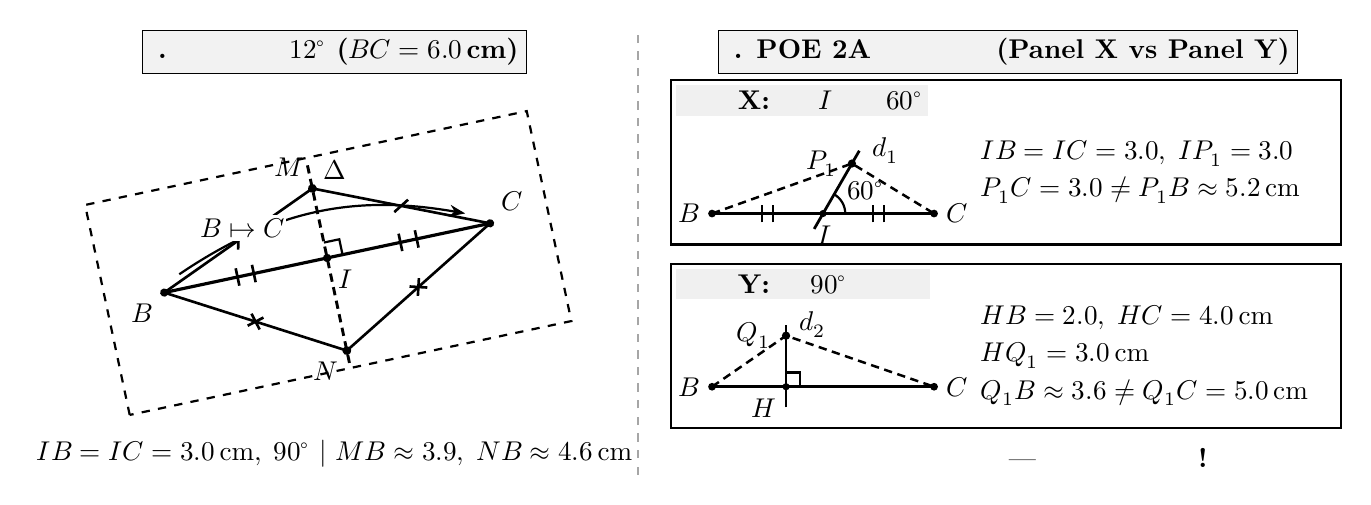
\begin{tikzpicture}[x=0.94cm, y=0.94cm, every node/.style={font=\linespread{1.0}\fontsize{9.8pt}{13.5pt}\selectfont, text=black}]
  \draw[line width=0.6pt, dashed, gray!70] (8.10, 0.05) -- (8.10, 6.08);
  \node[anchor=north, fill=headgray, draw=black, line width=0.5pt, inner sep=2.8pt] at (4.00, 6.06) {\textbf{ក. បត់បន្ទះទ្រេត $12^\circ$ \en{($BC=6.0\unit{cm}$)}}};
  \node[anchor=north, fill=headgray, draw=black, line width=0.5pt, inner sep=2.8pt] at (13.10, 6.06) {\textbf{ខ. \en{POE 2A}៖ សោតែ ១ ម្ខាង (\en{Panel X} \en{vs} \en{Panel Y})}};

  % Left Panel: Tilted 12 deg Paper Fold (BC=6.0 cm, M=2.5 cm, N=3.5 cm)
  \begin{scope}[shift={(3.90, 2.98)}, rotate=12]
    \draw[black, dashed, line width=0.8pt] (-3.05, -1.52) rectangle (3.05, 1.38);
    \coordinate (B) at (-2.25, 0);
    \coordinate (C) at (2.25, 0);
    \coordinate (I) at (0, 0);
    \coordinate (M) at (0, 0.96);
    \coordinate (N) at (0, -1.28);
    \draw[black, line width=1.15pt, tk2] (B) -- (I);
    \draw[black, line width=1.15pt, tk2] (I) -- (C);
    \draw[black, line width=1.05pt, densely dashed] (0, -1.45) -- (0, 1.28);
    \draw[black, line width=0.95pt, tkslash] (M) -- (B);
    \draw[black, line width=0.95pt, tkslash] (M) -- (C);
    \draw[black, line width=0.95pt, tkcross] (N) -- (B);
    \draw[black, line width=0.95pt, tkcross] (N) -- (C);
    \rightanglemark[0.20]{(I)}{(M)}{(C)}
    \draw[black, line width=0.8pt, -{Stealth[length=2mm]}, bend left=22] (-2.00, 0.20) to (1.95, 0.20);
    \node[fill=white, inner sep=1pt] at (-1.25, 0.68) {បត់ $B\mapsto C$};
    \fill[black] (B) circle (1.5pt) node[below left=1pt] {\en{$B$}};
    \fill[black] (C) circle (1.5pt) node[above right=1pt] {\en{$C$}};
    \fill[black] (I) circle (1.5pt) node[below right=1pt] {\en{$I$}};
    \fill[black] (M) circle (1.6pt) node[above left=1pt] {\en{$M$}};
    \fill[black] (N) circle (1.6pt) node[below left=1pt] {\en{$N$}};
    \node[right=2pt] at (0, 1.22) {\en{$\Delta$}};
  \end{scope}
  \node[anchor=south, align=center] at (4.00, 0.02) {\en{$IB=IC=3.0\unit{cm},\; 90^\circ$} $\vert$ \en{$MB\approx 3.9,\; NB\approx 4.6\unit{cm}$}};

  % Right Panel: POE 2A Panel X (top) and Panel Y (bottom)
  % Panel X: 60 deg slanted d1 through I
  \begin{scope}[shift={(8.55, 3.16)}]
    \draw[black, line width=0.85pt] (0, 0) rectangle (9.05, 2.22);
    \node[anchor=north west, fill=panelgray, inner sep=2pt] at (0.06, 2.16) {\textbf{ផ្ទាំង \en{X}:} កាត់ $I$ ទ្រេត $60^\circ$};
    \coordinate (XB) at (0.55, 0.42);
    \coordinate (XC) at (3.55, 0.42);
    \coordinate (XI) at (2.05, 0.42);
    \coordinate (XP1) at ($(XI)+(60:0.78)$);
    \draw[black, line width=1.1pt, tk2] (XB) -- (XI);
    \draw[black, line width=1.1pt, tk2] (XI) -- (XC);
    \draw[black, line width=1.0pt] ($(XI)+(-120:0.24)$) -- ($(XI)+(60:0.98)$) node[right=1pt] {\en{$d_1$}};
    \draw[black, densely dashed, line width=0.9pt] (XB) -- (XP1) -- (XC);
    \draw[ang1] ($(XI)+(0:0.30)$) arc (0:60:0.30);
    \node at ($(XI)+(28:0.65)$) {\en{$60^\circ$}};
    \fill[black] (XB) circle (1.4pt) node[left=1pt] {\en{$B$}};
    \fill[black] (XC) circle (1.4pt) node[right=1pt] {\en{$C$}};
    \fill[black] (XI) circle (1.3pt) node[below=1pt] {\en{$I$}};
    \fill[black] (XP1) circle (1.5pt) node[left=2pt] {\en{$P_1$}};
    \node[anchor=west, align=left] at (4.05, 0.98) {\en{$IB=IC=3.0,\; IP_1=3.0$}\\ \en{$P_1C=3.0 \neq P_1B\approx 5.2\unit{cm}$}};
  \end{scope}

  % Panel Y: Off-center perp d2 at H (HB=2.0, HC=4.0)
  \begin{scope}[shift={(8.55, 0.68)}]
    \draw[black, line width=0.85pt] (0, 0) rectangle (9.05, 2.22);
    \node[anchor=north west, fill=panelgray, inner sep=2pt] at (0.06, 2.16) {\textbf{ផ្ទាំង \en{Y}:} កែង $90^\circ$ ខុសកណ្ដាល};
    \coordinate (YB) at (0.55, 0.56);
    \coordinate (YC) at (3.55, 0.56);
    \coordinate (YH) at (1.55, 0.56);
    \coordinate (YQ1) at (1.55, 1.25);
    \draw[black, line width=1.1pt] (YB) -- (YC);
    \draw[black, line width=1.0pt] (1.55, 0.28) -- (1.55, 1.40) node[right=1pt] {\en{$d_2$}};
    \draw[black, densely dashed, line width=0.9pt] (YB) -- (YQ1) -- (YC);
    \rightanglemark[0.18]{(YH)}{(YC)}{(YQ1)}
    \fill[black] (YB) circle (1.4pt) node[left=1pt] {\en{$B$}};
    \fill[black] (YC) circle (1.4pt) node[right=1pt] {\en{$C$}};
    \fill[black] (YH) circle (1.3pt) node[below left=1pt] {\en{$H$}};
    \fill[black] (YQ1) circle (1.5pt) node[left=2pt] {\en{$Q_1$}};
    \node[anchor=west, align=left] at (4.05, 0.98) {\en{$HB=2.0,\; HC=4.0\unit{cm}$}\\ \en{$HQ_1=3.0\unit{cm}$}\\ \en{$Q_1B\approx 3.6 \neq Q_1C=5.0\unit{cm}$}};
  \end{scope}
  \node[anchor=south] at (13.10, 0.02) {សោតែ ១ ម្ខាងមិនគ្រប់គ្រាន់\en{---}ត្រូវការ\textbf{សោភ្លោះទាំង ២!}};
\end{tikzpicture}\par
\vspace{2pt}
{\fontsize{10.5pt}{14pt}\selectfont\textbf{រូបទី ១៖} ការបត់ក្រដាស \en{1:1} បន្ទះទ្រេត $12^\circ$ និងពិសោធន៍ \en{POE 2A} បង្ហាញការបរាជ័យនៃសោតែម្ខាង \en{(Coad, 2006; Catman-Aksoy \& Isiksal-Bostan, 2024; Hodancı \& Hacısalihoğlu Karadeniz, 2025)}។}
\end{tcolorbox}

% --- រូបទី ២ ---
\Needspace{7.2cm}
\begin{tcolorbox}[enhanced, sharp corners, colback=white, colframe=black, boxrule=0.8pt, top=5pt, bottom=4pt, left=4pt, right=4pt, before skip=4pt, after skip=6pt]
\centering
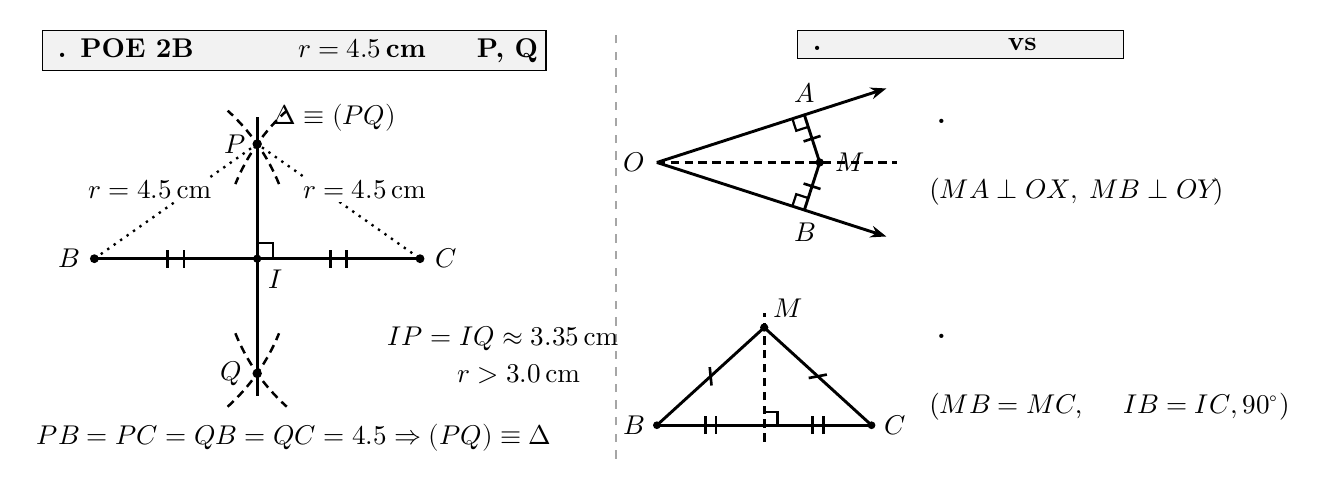
\begin{tikzpicture}[x=0.94cm, y=0.94cm, every node/.style={font=\linespread{1.0}\fontsize{9.8pt}{13.5pt}\selectfont, text=black}]
  \draw[line width=0.6pt, dashed, gray!70] (8.60, 0.05) -- (8.60, 5.86);
  \node[anchor=north, fill=headgray, draw=black, line width=0.5pt, inner sep=2.8pt] at (4.25, 5.84) {\textbf{ក. \en{POE 2B}៖ ធ្នូដែកឈាន $r=4.5\unit{cm}$ កាត់ \en{P, Q}}};
  \node[anchor=north, fill=headgray, draw=black, line width=0.5pt, inner sep=2.8pt] at (13.25, 5.84) {\textbf{ខ. ញែកសំណុំចំណុច៖ ពុះមុំ \en{vs} មេដ្យាទ័រ}};

  % Left Panel: POE 2B Dual-Arc Compass Construction
  \coordinate (B2) at (1.55, 2.75);
  \coordinate (C2) at (5.95, 2.75);
  \coordinate (I2) at (3.75, 2.75);
  \coordinate (P2) at (3.75, 4.30);
  \coordinate (Q2) at (3.75, 1.20);
  \draw[black, line width=1.2pt, tk2] (B2) -- (I2);
  \draw[black, line width=1.2pt, tk2] (I2) -- (C2);
  \draw[black, line width=1.05pt] (3.75, 0.90) -- (3.75, 4.66) node[right=2pt] {\en{$\Delta \equiv (PQ)$}};
  \draw[black, densely dashed, line width=0.9pt] ($(B2)+(22:2.691)$) arc (22:48:2.691);
  \draw[black, densely dashed, line width=0.9pt] ($(B2)+(-48:2.691)$) arc (-48:-22:2.691);
  \draw[black, densely dashed, line width=0.9pt] ($(C2)+(132:2.691)$) arc (132:158:2.691);
  \draw[black, densely dashed, line width=0.9pt] ($(C2)+(-158:2.691)$) arc (-158:-132:2.691);
  \draw[black, dotted, line width=0.85pt] (B2) -- (P2) -- (C2);
  \rightanglemark[0.20]{(I2)}{(C2)}{(P2)}
  \fill[black] (B2) circle (1.6pt) node[left=2pt] {\en{$B$}};
  \fill[black] (C2) circle (1.6pt) node[right=2pt] {\en{$C$}};
  \fill[black] (I2) circle (1.5pt) node[below right=1pt] {\en{$I$}};
  \fill[black] (P2) circle (1.7pt) node[left=2pt] {\en{$P$}};
  \fill[black] (Q2) circle (1.7pt) node[left=2pt] {\en{$Q$}};
  \node[fill=white, inner sep=1pt] at (2.30, 3.68) {\en{$r=4.5\unit{cm}$}};
  \node[fill=white, inner sep=1pt] at (5.20, 3.68) {\en{$r=4.5\unit{cm}$}};
  \node[anchor=west, align=left] at (5.38, 1.45) {\en{$IP=IQ\approx 3.35\unit{cm}$}\\ ត្រូវការ \en{$r > 3.0\unit{cm}$}};
  \node[anchor=south] at (4.25, 0.02) {\en{$PB=PC=QB=QC=4.5 \Rightarrow (PQ)\equiv\Delta$}};

  % Right Panel: Angle Bisector vs Perpendicular Bisector
  \begin{scope}[shift={(9.15, 3.20)}]
    \coordinate (O3) at (0, 0.85);
    \coordinate (X3) at (3.10, 1.85);
    \coordinate (Y3) at (3.10, -0.15);
    \coordinate (M3) at (2.20, 0.85);
    \coordinate (A3) at ($(O3)!(M3)!(X3)$);
    \coordinate (B3) at ($(O3)!(M3)!(Y3)$);
    \draw[black, line width=1.05pt, -{Stealth[length=2mm]}] (O3) -- (X3);
    \draw[black, line width=1.05pt, -{Stealth[length=2mm]}] (O3) -- (Y3);
    \draw[black, densely dashed, line width=0.95pt] (O3) -- (3.25, 0.85);
    \draw[black, line width=1.05pt, tk1] (M3) -- (A3);
    \draw[black, line width=1.05pt, tk1] (M3) -- (B3);
    \rightanglemark[0.16]{(A3)}{(O3)}{(M3)}
    \rightanglemark[0.16]{(B3)}{(O3)}{(M3)}
    \fill[black] (M3) circle (1.5pt) node[right=2pt] {\en{$M$}};
    \node[left=1pt] at (O3) {\en{$O$}};
    \node[above=1pt] at (A3) {\en{$A$}};
    \node[below=1pt] at (B3) {\en{$B$}};
    \node[anchor=west, align=left] at (3.55, 0.85) {\textbf{១. ពុះមុំ៖}\\ស្មើចម្ងាយ\textbf{កែងទៅជ្រុង ២}\\(\en{$MA\perp OX,\; MB\perp OY$})};
  \end{scope}

  \begin{scope}[shift={(9.15, 0.50)}]
    \coordinate (B4) at (0, 0);
    \coordinate (C4) at (2.90, 0);
    \coordinate (I4) at (1.45, 0);
    \coordinate (M4) at (1.45, 1.32);
    \draw[black, line width=1.1pt, tk2] (B4) -- (I4);
    \draw[black, line width=1.1pt, tk2] (I4) -- (C4);
    \draw[black, densely dashed, line width=0.95pt] (1.45, -0.22) -- (1.45, 1.52);
    \draw[black, line width=1.05pt, tkslash] (M4) -- (B4);
    \draw[black, line width=1.05pt, tkslash] (M4) -- (C4);
    \rightanglemark[0.17]{(I4)}{(C4)}{(M4)}
    \fill[black] (B4) circle (1.4pt) node[left=1pt] {\en{$B$}};
    \fill[black] (C4) circle (1.4pt) node[right=1pt] {\en{$C$}};
    \fill[black] (M4) circle (1.5pt) node[above right=0pt] {\en{$M$}};
    \node[anchor=west, align=left] at (3.55, 0.65) {\textbf{២. មេដ្យាទ័រ៖}\\ស្មើចម្ងាយ\textbf{ទៅចុង ២}\\(\en{$MB=MC$}, ដោយ $IB=IC, 90^\circ$)};
  \end{scope}
\end{tikzpicture}\par
\vspace{2pt}
{\fontsize{10.5pt}{14pt}\selectfont\textbf{រូបទី ២៖} ការសង់ធ្នូដែកឈាន \en{POE 2B ($r=4.5\unit{cm}$)} កំណត់ $(PQ)\equiv\Delta$ និងការញែកពុះមុំពីមេដ្យាទ័រ \en{(Chen et al., 2017; Demiray et al., 2023; Hodancı \& Hacısalihoğlu Karadeniz, 2025)}។}
\end{tcolorbox}

% --- រូបទី ៣ ---
\Needspace{7.2cm}
\begin{tcolorbox}[enhanced, sharp corners, colback=white, colframe=black, boxrule=0.8pt, top=5pt, bottom=4pt, left=4pt, right=4pt, before skip=4pt, after skip=6pt]
\centering
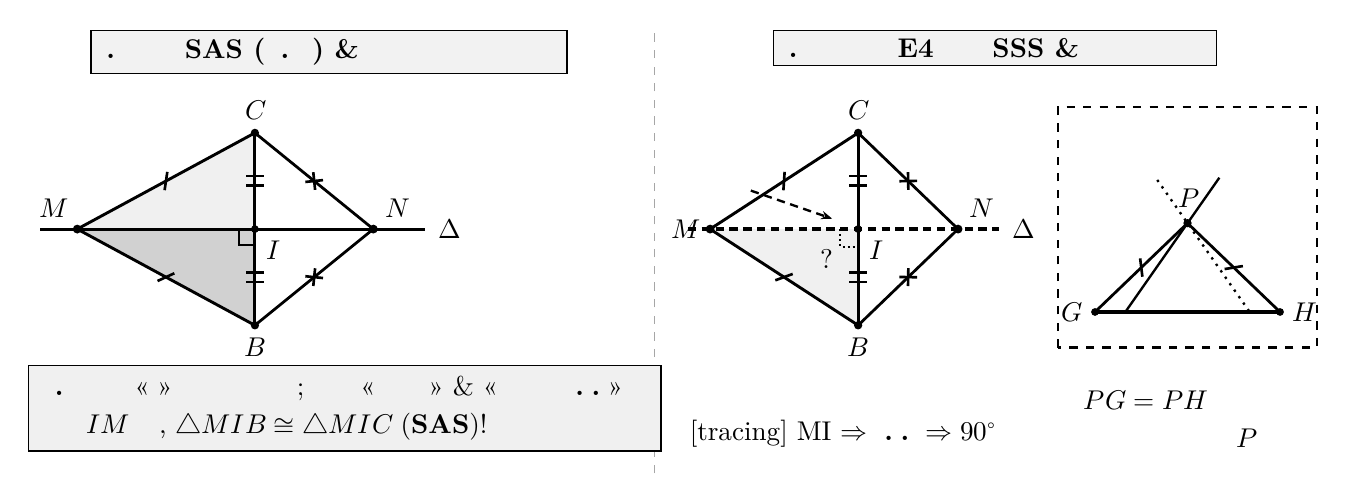
\begin{tikzpicture}[x=0.94cm, y=0.94cm, every node/.style={font=\linespread{1.0}\fontsize{9.8pt}{13.5pt}\selectfont, text=black}]
  \draw[line width=0.6pt, dashed, gray!70] (8.65, 0.05) -- (8.65, 6.06);
  \node[anchor=north, fill=headgray, draw=black, line width=0.5pt, inner sep=2.8pt] at (4.25, 6.04) {\textbf{ក. ផ្ទាល់ \en{SAS} (ទំ.១៥៦) \& កំណត់សម្គាល់អក្ខរាវិរុទ្ធ}};
  \node[anchor=north, fill=headgray, draw=black, line width=0.5pt, inner sep=2.8pt] at (13.25, 6.04) {\textbf{ខ. លំហាត់គំរូ \en{E4} ច្រាស \en{SSS} \& អន្ទាក់ ១ ចំណុច}};

  % Left Panel: Book p.156 vertical BC, horizontal Delta + errata callout
  \coordinate (B5) at (3.25, 2.05);
  \coordinate (C5) at (3.25, 4.65);
  \coordinate (I5) at (3.25, 3.35);
  \coordinate (M5) at (0.85, 3.35);
  \coordinate (N5) at (4.85, 3.35);
  \fill[panelgray] (M5) -- (C5) -- (I5) -- cycle;
  \fill[midgray] (M5) -- (I5) -- (B5) -- cycle;
  \draw[black, line width=1.15pt, tk2] (C5) -- (I5);
  \draw[black, line width=1.15pt, tk2] (I5) -- (B5);
  \draw[black, line width=1.05pt] (0.35, 3.35) -- (5.55, 3.35) node[right=1pt] {\en{$\Delta$}};
  \draw[black, line width=1.05pt, tkslash] (M5) -- (C5);
  \draw[black, line width=1.05pt, tkslash] (M5) -- (B5);
  \draw[black, line width=1.0pt, tkcross] (N5) -- (C5);
  \draw[black, line width=1.0pt, tkcross] (N5) -- (B5);
  \rightanglemark[0.20]{(I5)}{(M5)}{(B5)}
  \fill[black] (C5) circle (1.5pt) node[above=1pt] {\en{$C$}};
  \fill[black] (B5) circle (1.5pt) node[below=1pt] {\en{$B$}};
  \fill[black] (I5) circle (1.4pt) node[below right=1pt] {\en{$I$}};
  \fill[black] (M5) circle (1.6pt) node[above left=1pt] {\en{$M$}};
  \fill[black] (N5) circle (1.6pt) node[above right=1pt] {\en{$N$}};

  \node[anchor=north west, draw=black, fill=panelgray, line width=0.65pt, inner sep=4pt, align=left, text width=7.75cm] at (0.18, 1.52) {%
    \textbf{ទំ.១៥៦៖} ថែម «\textbf{។}» ចុងទ្រឹស្ដីទី ១; ឯកភាព «\textbf{ស្ថិតនៅ}» \en{\&} «\textbf{លក្ខខណ្ឌ ជ.ម.ជ}»។ ស្រាយ $IM$ រួម, $\tri{MIB}\cg\tri{MIC}$ (\textbf{SAS})!};

  % Right Panel: E4 Converse SSS (MI dashed + [tracing]) + 1-point trap
  \begin{scope}[shift={(9.05, 0.25)}]
    \coordinate (Ce) at (2.35, 4.40);
    \coordinate (Be) at (2.35, 1.80);
    \coordinate (Ie) at (2.35, 3.10);
    \coordinate (Me) at (0.35, 3.10);
    \coordinate (Ne) at (3.70, 3.10);
    \fill[panelgray] (Me) -- (Ie) -- (Be) -- cycle;
    \draw[black, line width=1.15pt, tk2] (Ce) -- (Ie);
    \draw[black, line width=1.15pt, tk2] (Ie) -- (Be);
    \draw[black, densely dashed, line width=1.15pt] (0.05, 3.10) -- (4.25, 3.10) node[right=1pt] {\en{$\Delta$}};
    \draw[black, line width=1.05pt, tkslash] (Me) -- (Ce);
    \draw[black, line width=1.05pt, tkslash] (Me) -- (Be);
    \draw[black, line width=1.0pt, tkcross] (Ne) -- (Ce);
    \draw[black, line width=1.0pt, tkcross] (Ne) -- (Be);
    \draw[black, densely dotted, line width=0.8pt] ($(Ie)+(-0.24,0)$) -- ($(Ie)+(-0.24,-0.24)$) -- ($(Ie)+(0,-0.24)$);
    \node at ($(Ie)+(-0.42,-0.40)$) {\en{$?$}};
    \draw[hypArrow] ($(Me)+(0.55,0.52)$) -- ($(Ie)+(-0.35,0.14)$);
    \fill[black] (Ce) circle (1.5pt) node[above=1pt] {\en{$C$}};
    \fill[black] (Be) circle (1.5pt) node[below=1pt] {\en{$B$}};
    \fill[black] (Ie) circle (1.4pt) node[below right=1pt] {\en{$I$}};
    \fill[black] (Me) circle (1.6pt) node[left=1pt] {\en{$M$}};
    \fill[black] (Ne) circle (1.6pt) node[above right=1pt] {\en{$N$}};
    \node[anchor=south] at (2.15, 0.02) {\en{[tracing] MI} $\Rightarrow$ \textbf{ជ.ជ.ជ} $\Rightarrow 90^\circ$};

    % 1-point trap subbox on far right
    \draw[black, dashed, line width=0.8pt] (5.05, 1.50) rectangle (8.55, 4.75);
    \node[anchor=north] at (6.80, 4.70) {\textbf{អន្ទាក់ ១ ចំណុច}};
    \coordinate (Gp) at (5.55, 1.98);
    \coordinate (Hp) at (8.05, 1.98);
    \coordinate (Pp) at (6.80, 3.18);
    \draw[black, line width=1.1pt] (Gp) -- (Hp);
    \draw[black, line width=1.0pt, tkslash] (Pp) -- (Gp);
    \draw[black, line width=1.0pt, tkslash] (Pp) -- (Hp);
    \draw[black, line width=0.85pt] ($(Pp)+(-125:1.45)$) -- ($(Pp)+(55:0.75)$);
    \draw[black, dotted, line width=0.85pt] ($(Pp)+(-55:1.45)$) -- ($(Pp)+(125:0.75)$);
    \fill[black] (Gp) circle (1.4pt) node[left=1pt] {\en{$G$}};
    \fill[black] (Hp) circle (1.4pt) node[right=1pt] {\en{$H$}};
    \fill[black] (Pp) circle (1.5pt) node[above=2pt] {\en{$P$}};
    \node[anchor=south, align=center] at (6.80, 0.02) {\en{$PG=PH$} មានបន្ទាត់\\ទ្រេតច្រើនកាត់ \en{$P$}};
  \end{scope}
\end{tikzpicture}\par
\vspace{2pt}
{\fontsize{10.5pt}{14pt}\selectfont\textbf{រូបទី ៣៖} សម្រាយផ្ទាល់ \en{SAS} និងកំណត់សម្គាល់ទំ.១៥៦ (ឆ្វេង) ទល់នឹងសម្រាយច្រាស \en{SSS} \en{E4} និងអន្ទាក់ ១ ចំណុច (ស្ដាំ) \en{(Muzaini et al., 2023; Winer \& Battista, 2022; Yeo \& Tzeng, 2019; Miyazaki et al., 2019)}។}
\end{tcolorbox}

% --- រូបទី ៤ ---
\Needspace{7.4cm}
\begin{tcolorbox}[enhanced, sharp corners, colback=white, colframe=black, boxrule=0.8pt, top=5pt, bottom=4pt, left=4pt, right=4pt, before skip=4pt, after skip=6pt]
\centering
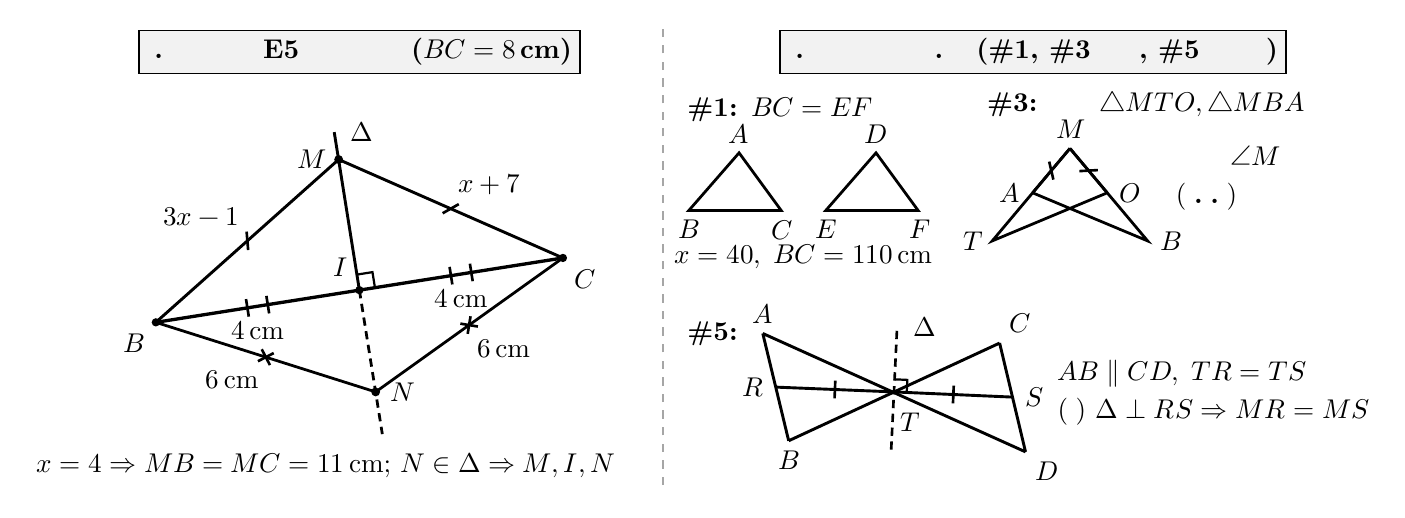
\begin{tikzpicture}[x=0.94cm, y=0.94cm, every node/.style={font=\linespread{1.0}\fontsize{9.8pt}{13.5pt}\selectfont, text=black}]
  \draw[line width=0.6pt, dashed, gray!70] (8.10, 0.05) -- (8.10, 6.22);
  \node[anchor=north, fill=headgray, draw=black, line width=0.5pt, inner sep=2.8pt] at (4.00, 6.20) {\textbf{ក. ប្រតិបត្តិ \en{E5}៖ ស្ថានីយសូឡា \en{($BC=8\unit{cm}$)}}};
  \node[anchor=north, fill=headgray, draw=black, line width=0.5pt, inner sep=2.8pt] at (13.10, 6.20) {\textbf{ខ. កិច្ចការផ្ទះ ទំ.១៦៤ (\en{\#1, \#3} បំបែក, \en{\#5} ២ ជំហាន)}};

  % Left Panel: E5 Practice Solar Station BC=8 cm, M(3x-1, x+7), N(6, 6)
  \coordinate (Bs) at (1.25, 2.25);
  \coordinate (Cs) at (6.75, 3.12);
  \coordinate (Is) at (4.00, 2.685);
  \coordinate (Ms) at (3.72, 4.45);
  \coordinate (Ns) at (4.22, 1.31);
  \draw[black, line width=1.2pt, tk2] (Bs) -- (Is);
  \draw[black, line width=1.2pt, tk2] (Is) -- (Cs);
  \draw[black, line width=1.05pt] (Is) -- (3.66, 4.82) node[right=2pt] {\en{$\Delta$}};
  \draw[black, densely dashed, line width=1.0pt] (Is) -- (4.31, 0.74);
  \rightanglemark[0.20]{(Is)}{(Cs)}{(Ms)}
  \draw[black, line width=1.05pt, tkslash] (Ms) -- (Bs);
  \draw[black, line width=1.05pt, tkslash] (Ms) -- (Cs);
  \draw[black, line width=1.0pt, tkcross] (Ns) -- (Bs);
  \draw[black, line width=1.0pt, tkcross] (Ns) -- (Cs);
  \fill[black] (Bs) circle (1.5pt) node[below left=1pt] {\en{$B$}};
  \fill[black] (Cs) circle (1.5pt) node[below right=1pt] {\en{$C$}};
  \fill[black] (Is) circle (1.5pt) node[above left=2pt] {\en{$I$}};
  \fill[black] (Ms) circle (1.6pt) node[left=2pt] {\en{$M$}};
  \fill[black] (Ns) circle (1.6pt) node[right=2pt] {\en{$N$}};
  \node[above left=1pt] at ($(Bs)!0.52!(Ms)$) {\en{$3x-1$}};
  \node[above right=1pt] at ($(Cs)!0.52!(Ms)$) {\en{$x+7$}};
  \node[below left=1pt] at ($(Bs)!0.52!(Ns)$) {\en{$6\unit{cm}$}};
  \node[below right=1pt] at ($(Cs)!0.52!(Ns)$) {\en{$6\unit{cm}$}};
  \node[below=2pt] at ($(Bs)!0.50!(Is)$) {\en{$4\unit{cm}$}};
  \node[below=2pt] at ($(Is)!0.50!(Cs)$) {\en{$4\unit{cm}$}};
  \node[anchor=south, align=center] at (4.00, 0.02) {\en{$x=4 \Rightarrow MB=MC=11\unit{cm}$}; \en{$N\in\Delta \Rightarrow M,I,N$} ត្រង់ជួរ};

  % Right Panel: HW #1, #3 (overlapped V + exploded), #5 (bowtie NO polygon fill + Delta perp RS)
  % #1 at top-left of right panel
  \begin{scope}[shift={(8.45, 3.62)}]
    \node[anchor=west] at (-0.15, 1.50) {\textbf{\en{\#1:} $BC=EF$}};
    \coordinate (b1) at (0.0, 0.14); \coordinate (c1) at (1.25, 0.14); \coordinate (a1) at (0.68, 0.92);
    \draw[black, line width=1.0pt] (a1) -- (b1) -- (c1) -- cycle;
    \node[above=0pt] at (a1) {\en{$A$}}; \node[below=0pt] at (b1) {\en{$B$}}; \node[below=0pt] at (c1) {\en{$C$}};
    \coordinate (e1) at (1.85, 0.14); \coordinate (f1) at (3.10, 0.14); \coordinate (d1) at (2.53, 0.92);
    \draw[black, line width=1.0pt] (d1) -- (e1) -- (f1) -- cycle;
    \node[above=0pt] at (d1) {\en{$D$}}; \node[below=0pt] at (e1) {\en{$E$}}; \node[below=0pt] at (f1) {\en{$F$}};
    \node[anchor=north] at (1.55, -0.18) {\en{$x=40,\; BC=110\unit{cm}$}};
  \end{scope}

  % #3 at top-right of right panel (overlapped V + exploded silhouettes)
  \begin{scope}[shift={(12.55, 3.35)}]
    \node[anchor=west] at (-0.20, 1.85) {\textbf{\en{\#3:} បំបែក \en{$\tri{MTO},\tri{MBA}$}}};
    \coordinate (M3h) at (1.05, 1.25);
    \coordinate (T3h) at (0.0, 0.0); \coordinate (B3h) at (2.10, 0.0);
    \coordinate (A3h) at ($(M3h)!0.48!(T3h)$); \coordinate (O3h) at ($(M3h)!0.48!(B3h)$);
    \draw[black, line width=1.0pt] (M3h) -- (T3h) -- (O3h) (M3h) -- (B3h) -- (A3h);
    \draw[black, line width=1.0pt, tkslash] (M3h) -- (A3h);
    \draw[black, line width=1.0pt, tkslash] (M3h) -- (O3h);
    \node[above=0pt] at (M3h) {\en{$M$}}; \node[left=1pt] at (A3h) {\en{$A$}}; \node[right=1pt] at (O3h) {\en{$O$}};
    \node[left=1pt] at (T3h) {\en{$T$}}; \node[right=1pt] at (B3h) {\en{$B$}};
    \node[anchor=west, align=left] at (2.35, 0.85) {មុំរួម \en{$\ang{M}$}\\(\textbf{ជ.ម.ជ})};
  \end{scope}

  % #5 at bottom of right panel (bowtie AB // CD, TR=TS, NO polygon fills!)
  \begin{scope}[shift={(9.45, 0.65)}]
    \node[anchor=west] at (-1.15, 1.45) {\textbf{\en{\#5:}}};
    \coordinate (A5) at (0.0, 1.45); \coordinate (B5h) at (0.35, 0.0);
    \coordinate (C5h) at (3.20, 1.32); \coordinate (D5) at (3.55, -0.15);
    \coordinate (T5) at (1.775, 0.66);
    \coordinate (R5) at (0.175, 0.725); \coordinate (S5) at (3.375, 0.59);
    \draw[black, line width=1.05pt] (A5) -- (B5h) (C5h) -- (D5) (A5) -- (D5) (B5h) -- (C5h);
    \draw[black, line width=1.05pt, tk1] (R5) -- (T5);
    \draw[black, line width=1.05pt, tk1] (T5) -- (S5);
    \coordinate (Db5) at ($(T5)+(-0.04,-0.78)$);
    \coordinate (Dt5) at ($(T5)+(0.04,0.88)$);
    \draw[black, densely dashed, line width=0.95pt] (Db5) -- (Dt5) node[right=2pt] {\en{$\Delta$}};
    \rightanglemark[0.16]{(T5)}{(S5)}{(Dt5)}
    \node[above=0pt] at (A5) {\en{$A$}}; \node[below=0pt] at (B5h) {\en{$B$}};
    \node[above right=0pt] at (C5h) {\en{$C$}}; \node[below right=0pt] at (D5) {\en{$D$}};
    \node[left=1pt] at (R5) {\en{$R$}}; \node[right=1pt] at (S5) {\en{$S$}};
    \node[fill=white, inner sep=1pt] at ($(T5)+(-65:0.45)$) {\en{$T$}};
    \node[anchor=west, align=left] at (3.85, 0.65) {\en{$AB\parallel CD,\; TR=TS$}\\ (ខ) \en{$\Delta\perp RS \Rightarrow MR=MS$}};
  \end{scope}
\end{tikzpicture}\par
\vspace{2pt}
{\fontsize{10.5pt}{14pt}\selectfont\textbf{រូបទី ៤៖} ស្ថានីយបូមទឹកសូឡា \en{E5 ($BC=8\unit{cm}$)} និងគំនូសបំបែកលំហាត់កិច្ចការផ្ទះទំ.១៦៤ (\en{\#1, \#3, \#5}) \en{(Biber, 2020; Šipuš et al., 2022)}។}
\end{tcolorbox}

% ============================================================================
% ផ្នែកទី ៦៖ មគ្គុទ្ទេសក៍រៀបចំ និងប្រើប្រាស់សម្ភារៈបោះពុម្ព (Pages 1--6) & ចម្លើយពេញលេញ
% ============================================================================
\secbanner{ផ្នែកទី ៦៖ មគ្គុទ្ទេសក៍រៀបចំ និងប្រើប្រាស់សម្ភារៈបោះពុម្ព \enbf{(Pages 1--6)}}{Section 6: Printing Calibration (Actual Size 100\%), Cut-Out Preparation \& Complete Master Answer Keys}

\subsec{៦\enbf{.}១ ស្តង់ដារបោះពុម្ព \enbf{Actual Size 100\%} និងលំដាប់ចែកសន្លឹកកិច្ចការ}

\begin{enumerate}[leftmargin=0.65cm, itemsep=2.5pt]
  \item \textbf{ការកំណត់បោះពុម្ព \en{1:1} ដាច់ខាត (ទំព័រ ១)៖} បោះពុម្ពឯកសារ \en{Printable\_Materials\_PB.pdf} ដោយជ្រើស \textbf{\en{Scale: Actual Size 100\%}} (\emph{ហាមប្រើ} \en{Fit to Page / Shrink to Fit}) ហើយវាស់ផ្ទៀងបន្ទះក្រិត \textbf{\en{5.0 cm}} នៅខាងស្ដាំផ្នែកខាងលើទំព័រ ១ ដើម្បីធានាថា $BC=6.0\unit{cm}$, ចំណុច $M$ ($2.5\unit{cm}$), $N$ ($3.5\unit{cm}$), ផ្ទាំង \en{POE 2A}, និងធ្នូដែកឈាន $r=4.5\unit{cm}$ មានខ្នាត \en{1:1} ពិតប្រាកដ។
  \item \textbf{ទម្រង់សន្សំក្រដាស ស-ខ្មៅ (ទំព័រ ២--៦)៖} ទំព័រ ២ (កាត \en{E4}) និងទំព័រ ៣ (សន្លឹក \en{E5} ៣ តួនាទី) ជាទម្រង់ \en{2-up} (២ ប័ណ្ណ/សន្លឹកក្នុង ១ ទំព័រ \en{A4}), ទំព័រ ៤ (ផ្ទាំងយោងប្រចាំថ្នាក់ និងធនាគារ \cnum{1}--\cnum{5}) គួរបោះពុម្ពលើក្រដាសរឹង \en{180 gsm} បិទលើក្ដារខៀន, ទំព័រ ៥ ជាកាតត្រួតពិនិត្យ \en{A--D} \en{4-up} + ចម្លើយគ្រូ, និងទំព័រ ៦ ជាប័ណ្ណកិច្ចការផ្ទះ \en{4-up}។
  \item \textbf{ឧបករណ៍តុក្រុម ៣ នាក់៖} កន្ត្រៃ ១, បន្ទាត់ក្រិត \en{cm/mm} ១, រ៉ាព័រទ័រ ១, និងដែកឈាន ១ ក្នុងមួយក្រុម។ ចែកទំព័រ ១ ផ្កាប់ចុះក្រោមនៅនាទី ០០', ទំព័រ ២ នៅនាទី ២៨', ទំព័រ ៣ នៅនាទី ៣៨', បង្ហាញទំព័រ ៥ នៅនាទី ៤៤.៥', និងចែកទំព័រ ៦ នៅនាទី ៤៨'។
\end{enumerate}

\Needspace{5.5cm}
\subsec{៦\enbf{.}២ ចម្លើយគំរូពេញលេញសម្រាប់គ្រប់សន្លឹកកិច្ចការ និងលំហាត់ \enbf{(Pages 1--6 \& HW)}}

\Needspace{6.0cm}
\begingroup
\linespread{1.05}\fontsize{10.5pt}{15.5pt}\selectfont
\begin{longtable}{|L{2.95cm}|L{13.90cm}|}
\hline
\rowcolor{headgray}
\multicolumn{1}{|C{2.95cm}|}{\tblhead{សន្លឹក \enbf{/} លំហាត់}} &
\multicolumn{1}{C{13.90cm}|}{\tblhead{ចម្លើយគំរូផ្លូវការ និងពិន្ទុត្រួតពិនិត្យ \enbf{(Master Key)}}} \\
\hline
\endfirsthead
\hline
\rowcolor{headgray}
\multicolumn{1}{|C{2.95cm}|}{\tblhead{សន្លឹក \enbf{/} លំហាត់}} &
\multicolumn{1}{C{13.90cm}|}{\tblhead{ចម្លើយគំរូផ្លូវការ និងពិន្ទុត្រួតពិនិត្យ \enbf{(Master Key)}}} \\
\hline
\endhead
\hline
\endfoot
\hline
\endlastfoot
\textbf{ទំព័រ ១ (\en{E2})} \newline ស.១ បត់ក្រដាស \newline \en{BC = 6.0 cm} &
បត់ចំណុច $B$ ត្រួតលើ $C$ បង្កើតផ្នត់ $\Delta$ កាត់ $I$៖ $IB = IC = \mathbf{3.0\unit{cm}}$; $\ang{MIB} = \ang{MIC} = \mathbf{90^\circ}$។ ចំណុច $M$ ($IM = 2.5\unit{cm}$ លើ $I$)៖ $MB = MC \approx \mathbf{3.9\unit{cm}}$ ($\sqrt{3.0^2+2.5^2} \approx 3.91\unit{cm}$); ចំណុច $N$ ($IN = 3.5\unit{cm}$ ក្រោម $I$)៖ $NB = NC \approx \mathbf{4.6\unit{cm}}$ ($\sqrt{3.0^2+3.5^2} \approx 4.61\unit{cm}$)~។ \\
\hline
\textbf{ទំព័រ ១ (\en{E2})} \newline \en{POE 2A--2B} &
\textbf{\en{POE 2A}:} ផ្ទាំង \en{X} ($d_1$ កាត់ $I$ ទ្រេត $60^\circ, IP_1=3.0\unit{cm}$): $P_1C = \mathbf{3.0\unit{cm}} \neq P_1B \approx \mathbf{5.2\unit{cm}}$ (ខ្វះសោ $90^\circ$); ផ្ទាំង \en{Y} ($d_2\perp BC$ ត្រង់ $H, HB=2.0, HC=4.0, HQ_1=3.0\unit{cm}$): $Q_1B \approx \mathbf{3.6\unit{cm}} \neq Q_1C = \mathbf{5.0\unit{cm}}$ (ខ្វះសោ $IB=IC$) $\Rightarrow$ ត្រូវការ\textbf{សោភ្លោះទាំង ២}។ \newline
\textbf{\en{POE 2B}:} ធ្នូ $r=4.5\unit{cm}$ ពី $B, C$ កាត់ត្រង់ $P, Q$ ($PB=PC=QB=QC=4.5\unit{cm}$, $IP=IQ \approx 3.35\unit{cm}$) $\Rightarrow$ បន្ទាត់ $(PQ)$ កាត់ត្រង់ $I$ ($IB=IC=3.0\unit{cm}$) និង $\ang{PIB}=90^\circ \Rightarrow (PQ)\equiv\Delta$។ បើ $r \le 3.0\unit{cm}$ ធ្នូមិនកាត់គ្នា ២ ចំណុចទេ (ប៉ះគ្នាតែត្រង់ $I$ បើ $r=3$, មិនជួបគ្នាបើ $r<3$)។ \\
\hline
\textbf{ទំព័រ ២ (\en{E4})} \newline លំហាត់គំរូ \newline (បំពេញទំ.១៥៦) &
\textbf{(ក) ទ្រឹស្ដីច្រាស (\textbf{ជ.ជ.ជ}):} គូសជំនួយ $MI$ ដាច់ៗ។ ក្នុង $\tri{MIB}, \tri{MIC}$៖ ១) $IB=IC$ (\cnum{1} $I$ កណ្ដាល $BC$), ២) $MB=MC$ (បម្រាប់/កាំស្មើ), ៣) ជ្រុងរួម $IM=IM \Rightarrow \tri{MIB}\cg\tri{MIC}$ (\cnum{3} \textbf{ជ.ជ.ជ}) $\Rightarrow \ang{MIB}=\ang{MIC}$។ ដោយ $\ang{MIB}+\ang{MIC}=180^\circ \Rightarrow \ang{MIB}=\ang{MIC}=\mathbf{90^\circ}$ (\cnum{2}) $\Rightarrow (MI)\perp BC$ ត្រង់ $I \Rightarrow (MI)$ ជាមេដ្យាទ័រ $BC$ (\cnum{5})។ \newline
\textbf{(ខ) គោលការណ៍ ២ ចំណុច៖} $MB=MC \Rightarrow M\in\Delta$ និង $NB=NC \Rightarrow N\in\Delta$ (\cnum{5}); ២ ចំណុច $M\neq N$ កំណត់បន្ទាត់តែ ១ គត់ $\Rightarrow (MN)\equiv\Delta$ ដោយមិនបាច់វាស់ $I$។ \newline
\textbf{\en{EIA 30s}:} មានតែ ១ ចំណុច $P$ ($PB=PC$) មានបន្ទាត់ទ្រេតរាប់មិនអស់កាត់ $P$ មិនកំណត់ $\Delta$ ទេ។ \\
\hline
\textbf{ទំព័រ ៣ (\en{E5})} \newline ប្រតិបត្តិ \newline (សូឡា ៣ តួនាទី) &
\textbf{តួនាទី ១ (\en{Pause-Ask}):} គូស $90^\circ$, \ticktwo{} លើ $IB, IC$, \tickslash{} លើ $MB, MC$, \tickcross{} លើ $NB, NC$; ផ្ទៀង $I$ កណ្ដាល $BC$ និង $\Delta\perp BC$ ត្រង់ $I$។ \newline
\textbf{តួនាទី ២ (ក):} $I$ កណ្ដាល $BC=8\unit{cm}$ (\cnum{1}) $\Rightarrow IB=IC=\mathbf{4\unit{cm}}$; $\Delta\perp BC$ (\cnum{2}), $M\in\Delta \Rightarrow MB=MC$ (\cnum{4}); សមីការ $3x-1=x+7 \Rightarrow 2x=8 \Rightarrow \mathbf{x=4} \Rightarrow MB=MC=3(4)-1=\mathbf{11\unit{cm}}$។ \newline
\textbf{តួនាទី ៣ (\en{Pause-Review}, ខ):} ផ្ទៀង $3(4)-1=11$ និង $4+7=11\unit{cm}$។ ដោយ $NB=NC=6\unit{cm}$ (\cnum{5}) $\Rightarrow N\in\Delta \Rightarrow M, I, N$ \textbf{រួមបន្ទាត់ត្រង់} $\Delta$។ \textbf{បិទ \en{E1}:} ដាក់សូឡា $M$ ($11\unit{cm}$) ឬអាង $N$ ($6\unit{cm}$) លើទីទួល $\Delta\setminus\{I\}$ រួចផុតទឹកលិច និងស្មើចម្ងាយពី $B, C$។ \\
\hline
\textbf{ទំព័រ ៥} \newline (កាត \en{A--D}) &
\textbf{កាត \en{A} (\ding{51} ពិត, មេដៃឡើង):} $\Delta\perp AB$ ត្រង់ $I$ ($90^\circ$, \cnum{2}) និង $IA=IB=4\unit{cm}$ (\cnum{1}) $\Rightarrow MB=MA=\mathbf{5\unit{cm}}$ (\cnum{4}) ទោះទ្រេត $22^\circ$។ \newline
\textbf{កាត \en{B} (\ding{55} ខុស, ខ្វែងដៃ):} $IC=ID=3\unit{cm}$ តែខ្វះ $90^\circ$ ($\ang{MIC}=65^\circ\neq 90^\circ$) $\Rightarrow MC\neq MD$ (អន្ទាក់មេដ្យានទ្រេត)។ \newline
\textbf{កាត \en{C} (\ding{55} ខុស, ខ្វែងដៃ):} កែង $90^\circ$ ត្រង់ $H$ តែខុសកណ្ដាល ($HE=2\unit{cm}\neq HF=5\unit{cm}$) $\Rightarrow ME\neq MF$ (អន្ទាក់កែងខុសកណ្ដាល)។ \newline
\textbf{កាត \en{D} (\ding{55} ខុស, ខ្វែងដៃ):} ស្មើចម្ងាយតែ \textbf{១ ចំណុច} ($PG=PH=5\unit{cm}$), ឯ $d$ កាត់ $K$ ($KG=2\neq KH=4, d\not\perp GH$) មិនមែនមេដ្យាទ័រទេ! \\
\hline
\textbf{ទំព័រ ៦ (ផ្ទះ)} \newline ទំ.១៦៤ \newline \en{\#1, \#3, \#5} &
\textbf{លំហាត់ \en{\#1}:} $\tri{ABC}\cg\tri{DEF} \Rightarrow BC=EF \Rightarrow 2x+30=5x-90 \Rightarrow 3x=120 \Rightarrow \mathbf{x=40} \Rightarrow BC=2(40)+30=\mathbf{110\unit{cm}}$។ \newline
\textbf{លំហាត់ \en{\#3}:} ដកស្រង់ $\tri{MTO}$ និង $\tri{MBA}$៖ មាន $MT=MB$ (ប្រធាន\en{---}គ្មានគំនូសលើរូបទំ.១៦៤), មុំរួម $\ang{TMO}=\ang{BMA}$, $MO=MA$ (ប្រធាន) $\Rightarrow \tri{MTO}\cg\tri{MBA}$ (\textbf{ជ.ម.ជ / \en{SAS}})។ \newline
\textbf{លំហាត់ \en{\#5}:} \textbf{(ក)} ក្នុង $\tri{ART}, \tri{DST}$៖ $\ang{RAT}=\ang{SDT}$ (មុំឆ្លាស់ក្នុង $AB\parallel CD$), $TR=TS$ (ប្រធាន), $\ang{ATR}=\ang{DTS}$ (មុំទល់កំពូល) $\Rightarrow \tri{ART}\cg\tri{DST}$ (\textbf{ម.ជ.ម / \en{ASA}}) $\Rightarrow AT=DT$។ បន្តក្នុង $\tri{ABT}, \tri{DCT}$៖ $\ang{BAT}=\ang{CDT}$, $AT=DT$, $\ang{ATB}=\ang{DTC} \Rightarrow \tri{ABT}\cg\tri{DCT}$ (\textbf{ម.ជ.ម / \en{ASA}})។ \textbf{(ខ)} បន្ថែម៖ ដោយ $TR=TS$ (\cnum{1}) និង $\Delta\perp RS$ ត្រង់ $T$ (\cnum{2}) $\Rightarrow \Delta$ ជាមេដ្យាទ័រនៃ $RS$ (\cnum{4}) $\Rightarrow \mathbf{MR=MS}$! \newline
\textit{កំណត់សម្គាល់៖ លំហាត់ \en{\#2} ទំ.១៦៤ ត្រូវបានផ្ទេរទៅ \en{Slice 5} (២.២) ដើម្បីស្របតាមមូលដ្ឋានត្រីកោណសមបាទ។} \\
\hline
\end{longtable}
\endgroup

% ============================================================================
% ផ្នែកទី ៧៖ បញ្ជីឯកសារយោង (References --- APA 7th Edition) & ហត្ថលេខា
% ============================================================================
\vspace{10pt}
\secbanner{ផ្នែកទី ៧៖ បញ្ជីឯកសារយោង \enbf{(References --- APA 7th Edition)}}{Section 7: Verified Open-Access Reference List (100\% 1-to-1 Match with PDFs 01--14)}

{\TimesEn\linespread{1.0}\selectfont\fontsize{10.8pt}{16.2pt}\selectfont
\setlength{\parskip}{6.0pt}
\everypar={\hangindent=0.85cm \hangafter=1}

Bento, S., Ferreira, H., \& Hall, A. (2018). Voronoi diagrams: Didactical and artistic applications. In E. Torrence, B. Torrence, C. Séquin, \& K. Fenyvesi (Eds.), \textit{Proceedings of Bridges 2018: Mathematics, Art, Music, Architecture, Education, Culture} (pp. 355--358). Tessellations Publishing. \url{https://archive.bridgesmathart.org/2018/bridges2018-355.pdf}

Biber, A. Ç. (2020). Students' difficulties in similar triangle questions. \textit{Cypriot Journal of Educational Sciences}, \textit{15}(5), 1146--1159. \url{https://doi.org/10.18844/cjes.v15i5.5161}

Boz-Yaman, B. (2024). Effects of using patty paper practices during geometric constructions on attitude, self-efficacy, and achievement in geometry. \textit{Electronic Journal for Research in Science \& Mathematics Education}, \textit{28}(3), 1--15. \url{https://files.eric.ed.gov/fulltext/EJ1459697.pdf}

Catman-Aksoy, E., \& Isiksal-Bostan, M. (2024). Fostering students’ definitions and images in parallelism and perpendicularity: A paper folding activity. \textit{European Journal of Science and Mathematics Education}, \textit{12}(2), 236--257. \url{https://doi.org/10.30935/scimath/14360}

Chen, M.-J., Lee, C.-Y., Lei, K. H., Tso, T.-Y., \& Lin, S.-L. (2017). Multimedia instruction presented by integrated context to enhance understanding of compass-and-straightedge construction. \textit{EURASIA Journal of Mathematics, Science and Technology Education}, \textit{13}(7), 3735--3752. \url{https://doi.org/10.12973/eurasia.2017.00756a}

Coad, L. (2006). Paper folding in the middle school classroom and beyond. \textit{The Australian Mathematics Teacher}, \textit{62}(1), 6--13. \url{https://files.eric.ed.gov/fulltext/EJ743584.pdf}

Demiray, E., Işıksal-Bostan, M., \& Saygı, E. (2023). Components of collective argumentation in geometric construction tasks. \textit{Turkish Journal of Education}, \textit{12}(1), 50--71. \url{https://doi.org/10.19128/turje.1176981}

Hodancı, A. N., \& Hacısalihoğlu Karadeniz, M. (2025). The role of a brain game in eliminating misconceptions in geometry and measurement. \textit{Instructional Technology and Lifelong Learning}, \textit{6}(1), 43--76. \url{https://doi.org/10.52911/itall.1539069}

Krajcevski, M., \& Sears, R. (2019). Common visual representations as a source for misconceptions of preservice teachers in a geometry connection course. \textit{International Journal for Mathematics Teaching and Learning}, \textit{20}(1), 85--105. \url{https://doi.org/10.4256/ijmtl.v20i1.189}

Miyazaki, M., Nagata, J., Chino, K., Sasa, H., Fujita, T., Komatsu, K., \& Shimizu, S. (2019). Curriculum development for explorative proving in lower secondary school geometry: Focusing on the levels of planning and constructing a proof. \textit{Frontiers in Education}, \textit{4}, 31. \url{https://doi.org/10.3389/feduc.2019.00031}

Muzaini, M., Rahayuningsih, S., Ikram, M., \& Nasiruddin, F. A.-Z. (2023). Mathematical creativity: Student geometrical figure apprehension in geometry problem-solving using new auxiliary elements. \textit{International Journal of Educational Methodology}, \textit{9}(1), 139--150. \url{https://doi.org/10.12973/ijem.9.1.139}

Šipuš, Ž. M., Bašić, M., Doorman, M., Špalj, E., \& Antoliš, S. (2022). MERIA -- Conflict lines: Experience with two innovative teaching materials. \textit{Center for Educational Policy Studies Journal}, \textit{12}(1), 103--124. \url{https://doi.org/10.26529/cepsj.987}

Winer, M. L., \& Battista, M. T. (2022). Investigating students’ proof reasoning: Analyzing students’ oral proof explanations and their written proofs in high school geometry. \textit{International Electronic Journal of Mathematics Education}, \textit{17}(2), em0677. \url{https://doi.org/10.29333/iejme/11713}

Yeo, L.-M., \& Tzeng, Y.-T. (2019). Tracing effect in the worked examples-based learning: An exploration of individual differences in working memory capacity. \textit{EURASIA Journal of Mathematics, Science and Technology Education}, \textit{15}(10), em1760. \url{https://doi.org/10.29333/ejmste/105482}
\par}

\vspace{20pt}
\Needspace{4.5cm}
\hfill
\begin{minipage}{9.8cm}
  {\centering
    ថ្ងៃអង្គារ ៧រោច ខែកត្តិក ឆ្នាំមមី អដ្ឋស័ក ពុទ្ធសករាជ ២៥៧០\\[2pt]
    ត្រូវនឹងថ្ងៃទី១ ខែធ្នូ ឆ្នាំ២០២៦\\[3pt]
    {\muol គ្រូបង្រៀន}\par}
  \vspace{32pt}
  \hfill{\muol ហុក ប៊ុនថែន}\hspace*{1.4cm}
\end{minipage}

\end{document}
